% ============================================================
%  Network Security -- Module 5: Legal, Ethical and Policy Issues
%  Lesson 5: Key Escrow
%  Lesson 8: Legal Issues
%  Beamer (Madrid theme). Compile with: pdflatex module5.tex (twice)
% ============================================================
\documentclass[aspectratio=169,11pt,xcolor={table}]{beamer}
\usetheme{Madrid}
\usefonttheme{professionalfonts}

\usepackage[T1]{fontenc}
\usepackage{lmodern}
\usepackage{booktabs}
\usepackage{array}
\usepackage{tikz}
\usetikzlibrary{arrows.meta,positioning,shapes.geometric,shapes.symbols,
  shapes.misc,shadows,calc,fit,backgrounds,mindmap,decorations.pathmorphing,decorations.pathreplacing}

% ------------------------------------------------------------
%  Colour palette
% ------------------------------------------------------------
\definecolor{navy}{RGB}{21,45,99}
\definecolor{ocean}{RGB}{28,97,158}
\definecolor{aqua}{RGB}{0,142,150}
\definecolor{brick}{RGB}{200,55,45}
\definecolor{amber}{RGB}{235,150,20}
\definecolor{leaf}{RGB}{40,160,90}
\definecolor{grape}{RGB}{125,70,165}
\definecolor{sky}{RGB}{235,243,252}
\definecolor{ink}{RGB}{40,40,50}

\setbeamercolor{palette primary}{bg=ocean,fg=white}
\setbeamercolor{palette secondary}{bg=navy!85,fg=white}
\setbeamercolor{palette tertiary}{bg=navy,fg=white}
\setbeamercolor{palette quaternary}{bg=navy,fg=white}
\setbeamercolor{structure}{fg=ocean}
\setbeamercolor{title}{bg=navy,fg=white}
\setbeamercolor{frametitle}{bg=navy,fg=white}
\setbeamercolor{block title}{bg=ocean,fg=white}
\setbeamercolor{block body}{bg=sky,fg=ink}
\setbeamercolor{block title alerted}{bg=brick,fg=white}
\setbeamercolor{block body alerted}{bg=brick!8,fg=ink}
\setbeamercolor{block title example}{bg=leaf,fg=white}
\setbeamercolor{block body example}{bg=leaf!8,fg=ink}
\setbeamercolor{normal text}{fg=ink}
\setbeamercolor{alerted text}{fg=brick}
\setbeamercolor{item projected}{bg=ocean,fg=white}
\setbeamertemplate{items}[circle]
\setbeamertemplate{blocks}[rounded][shadow=true]
\setbeamertemplate{navigation symbols}{}

% Section divider slide
\AtBeginSection[]{
  \begin{frame}[plain]
    \begin{tikzpicture}[remember picture,overlay]
      \fill[navy] (current page.south west) rectangle (current page.north east);
      \fill[ocean] (current page.south west) rectangle ([yshift=1.2cm]current page.south east);
      \fill[aqua] ([yshift=1.2cm]current page.south west) rectangle ([yshift=1.35cm]current page.south east);
      \foreach \i in {1,...,6}
        \draw[white,opacity=0.06,line width=14pt]
          ([xshift=\i*1.6cm]current page.north west) circle (\i*0.9cm);
      \node[white,font=\large,anchor=west] at ([xshift=1.2cm,yshift=0.9cm]current page.west)
        {Lesson \thesection};
      \node[white,font=\huge\bfseries,anchor=west,text width=12cm] at ([xshift=1.2cm,yshift=-0.1cm]current page.west)
        {\insertsectionhead};
      \node[white,opacity=0.8,anchor=east,font=\small] at ([xshift=-0.8cm,yshift=0.6cm]current page.south east)
        {Module 5 \,$\cdot$\, Legal, Ethical and Policy Issues};
    \end{tikzpicture}
  \end{frame}
}

% ------------------------------------------------------------
%  TikZ styles and small pictograms
% ------------------------------------------------------------
\tikzset{
  >={Stealth[length=2.6mm]},
  box/.style={draw=#1!80!black,fill=#1!15,rounded corners=4pt,thick,
    minimum height=8mm,minimum width=22mm,align=center,font=\small,
    drop shadow={opacity=0.25}},
  box/.default=ocean,
  lay/.style={fill=#1,text=white,rounded corners=3pt,minimum width=38mm,minimum height=9mm,font=\scriptsize,align=center},
  solid box/.style={fill=#1,text=white,rounded corners=4pt,
    minimum height=8mm,minimum width=22mm,align=center,font=\small\bfseries,
    drop shadow={opacity=0.3}},
  solid box/.default=ocean,
  flow/.style={->,very thick,draw=#1},
  flow/.default=ink!70,
  station/.style={circle,draw=#1!80!black,fill=#1!20,very thick,minimum size=13mm,
    font=\small\bfseries,align=center},
  station/.default=ocean,
  tag/.style={font=\scriptsize,text=ink!80,align=center},
  layer/.style={draw=white,thick,fill=#1,text=white,minimum width=40mm,
    minimum height=6.5mm,font=\small\bfseries},
  % pictograms
  pics/pc/.style={code={
    \fill[#1!85!black,rounded corners=1.5pt] (-0.42,-0.05) rectangle (0.42,0.52);
    \fill[white!90!#1] (-0.36,0.01) rectangle (0.36,0.46);
    \fill[#1!85!black] (-0.06,-0.05) rectangle (0.06,-0.18);
    \fill[#1!85!black,rounded corners=1pt] (-0.24,-0.18) rectangle (0.24,-0.24);
  }},
  pics/pc/.default=ocean,
  pics/person/.style={code={
    \fill[#1] (0,0.46) circle (0.16);
    \fill[#1,rounded corners=5pt] (-0.27,-0.1) -- (-0.27,0.2) -- (0.27,0.2) -- (0.27,-0.1) -- cycle;
  }},
  pics/person/.default=ocean,
  pics/lock/.style={code={
    \draw[#1!80!black,line width=2.2pt] (-0.15,0.12) -- (-0.15,0.28) arc (180:0:0.15) -- (0.15,0.12);
    \fill[#1,rounded corners=2pt] (-0.26,-0.22) rectangle (0.26,0.14);
    \fill[white] (0,-0.02) circle (0.05);
    \fill[white] (-0.02,-0.02) rectangle (0.02,-0.13);
  }},
  pics/lock/.default=amber,
  pics/doc/.style={code={
    \fill[white,draw=#1,thick] (-0.25,-0.33) -- (-0.25,0.33) -- (0.12,0.33) -- (0.25,0.2) -- (0.25,-0.33) -- cycle;
    \draw[#1,thick] (0.12,0.33) -- (0.12,0.2) -- (0.25,0.2);
    \foreach \y in {0.12,0,-0.12,-0.24} \draw[#1!70,thick] (-0.16,\y) -- (0.16,\y);
  }},
  pics/doc/.default=ocean,
  pics/key/.style={code={
    \draw[#1,line width=2pt] (0,0) circle (0.12);
    \draw[#1,line width=2pt] (0.12,0) -- (0.5,0) (0.38,0) -- (0.38,-0.12) (0.47,0) -- (0.47,-0.1);
  }},
  pics/key/.default=amber,
}
\newcommand{\comma}{,}
\newcommand{\hl}[1]{\textcolor{ocean}{\textbf{#1}}}
\newcommand{\bad}[1]{\textcolor{brick}{\textbf{#1}}}
\newcommand{\good}[1]{\textcolor{leaf}{\textbf{#1}}}

\makeatletter
% University logo, small, top-right corner of every page
\AddToHook{shipout/foreground}{%
  \put(\strip@pt\paperwidth,0){%
    \makebox(0,0)[tr]{\raisebox{-0.8cm}{
\includegraphics[height=0.72cm]{au_logo.png}\hspace{0.15cm}}}}}
\makeatother

% ------------------------------------------------------------
\title[Module 5: Legal \& Policy]{Legal, Ethical and Policy Issues}
\subtitle{Module 5 \,\textbar\, Lesson 5: Key Escrow \,\textbullet\, Lesson 8: Legal Issues}
\author[Network Security]{Network Security}
\institute[SLM]{Self-Learning Material \,--\, Lessons 5 \& 8}
\date{}

% scales-of-justice pictogram
\tikzset{pics/scales/.style={code={
  \fill[#1] (-0.06,-0.7) rectangle (0.06,0.55);
  \fill[#1] (-0.35,-0.78) rectangle (0.35,-0.68);
  \draw[#1,line width=1.6pt] (-0.75,0.45) -- (0.75,0.45);
  \fill[#1] (0,0.6) circle (0.08);
  \foreach \s in {-1,1}{
    \draw[#1,thick] (\s*0.75,0.45) -- (\s*0.5,-0.05) (\s*0.75,0.45) -- (\s*1.0,-0.05);
    \fill[#1] (\s*0.47,-0.05) arc (180:360:0.28 and 0.14) -- cycle;
  }
}},pics/scales/.default=navy}

\begin{document}

% ============================================================
\begin{frame}[plain]
  
\begin{tikzpicture}[remember picture,overlay]
    \shade[top color=navy,bottom color=ocean] (current page.south west) rectangle (current page.north east);
    \foreach \i/\o in {1/0.10,2/0.08,3/0.06,4/0.05,5/0.04}
      \draw[white,opacity=\o,line width=1.2pt] ([xshift=-2.5cm,yshift=-0.5cm]current page.north east) circle (\i*1.1cm);
    \fill[aqua] ([yshift=2.35cm]current page.south west) rectangle ([yshift=2.45cm]current page.south east);
    \begin{scope}[shift={([xshift=-3.0cm,yshift=0.5cm]current page.east)},scale=1.7]
      \pic at (0,0) {scales=white};
      \pic[scale=0.45] at (-0.75,-0.3) {key=amber};
      \pic[scale=0.35] at (0.75,-0.25) {lock=amber};
    \end{scope}
    \node[white,anchor=west,font=\normalsize] at ([xshift=1.1cm,yshift=2.4cm]current page.west)
      {NETWORK SECURITY \,\textbar\, MODULE 5};
    \node[white,anchor=west,font=\fontsize{26}{31}\selectfont\bfseries,text width=10cm] at ([xshift=1.1cm,yshift=1.0cm]current page.west)
      {Legal, Ethical and\\[2pt] Policy Issues};
    \node[white,opacity=0.9,anchor=west,text width=9cm,font=\small] at ([xshift=1.1cm,yshift=-0.9cm]current page.west)
      {Lesson 5 \,--\, Key Escrow\\ Lesson 8 \,--\, Legal Issues};
    \node[white,opacity=0.85,anchor=west,font=\footnotesize] at ([xshift=1.1cm,yshift=1.2cm]current page.south west)
      {Key escrow \,$\cdot$\, Privacy \,$\cdot$\, Digital signatures \,$\cdot$\, IT Act 2000 \,$\cdot$\, Indian laws \,$\cdot$\, Patents};
  \end{tikzpicture}
\end{frame}

% ============================================================
\begin{frame}{Roadmap of This Module}
  \centering
  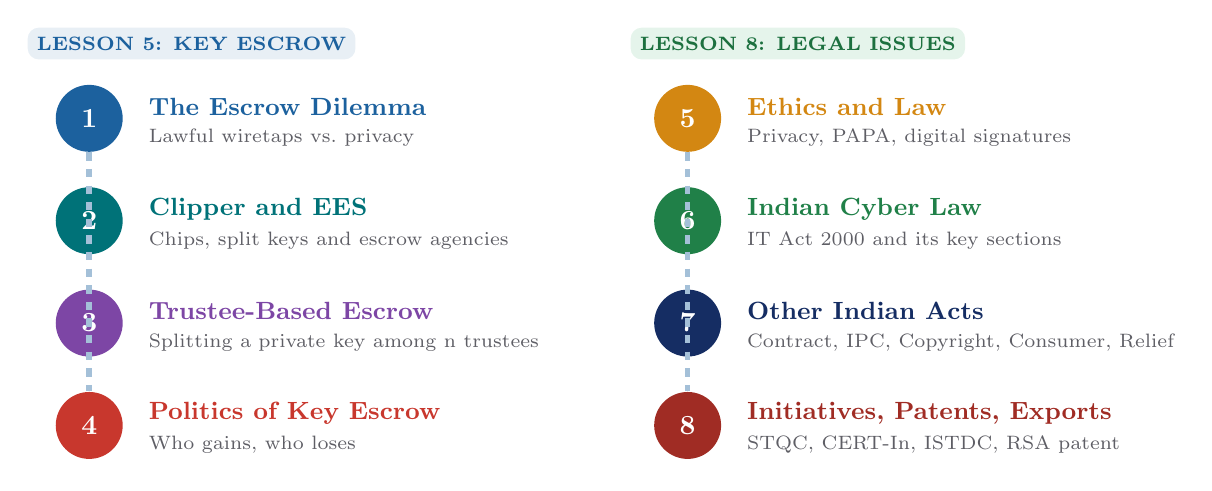
\begin{tikzpicture}
    \foreach \t/\c/\n [count=\i] in {
      The Escrow Dilemma/ocean/Lawful wiretaps vs.\ privacy,
      Clipper and EES/aqua!80!black/Chips\comma{} split keys and escrow agencies,
      Trustee-Based Escrow/grape/Splitting a private key among n trustees,
      Politics of Key Escrow/brick/Who gains\comma{} who loses,
      Ethics and Law/amber!90!black/Privacy\comma{} PAPA\comma{} digital signatures,
      Indian Cyber Law/leaf!80!black/IT Act 2000 and its key sections,
      Other Indian Acts/navy/Contract\comma{} IPC\comma{} Copyright\comma{} Consumer\comma{} Relief,
      Initiatives\comma{} Patents\comma{} Exports/brick!80!black/STQC\comma{} CERT-In\comma{} ISTDC\comma{} RSA patent}
    {
      \pgfmathsetmacro{\x}{ifthenelse(\i<5,0,7.6)}
      \pgfmathsetmacro{\y}{-mod(\i-1,4)*1.3}
      \node[circle,fill=\c,text=white,font=\bfseries,minimum size=8.5mm] (n\i) at (\x,\y) {\i};
      \node[anchor=west,font=\small\bfseries,text=\c] at ([xshift=2mm,yshift=1.5mm]n\i.east) {\t};
      \node[anchor=west,font=\scriptsize,text=ink!75] at ([xshift=2mm,yshift=-2.5mm]n\i.east) {\n};
    }
    \draw[ocean!40,line width=2pt,dashed] (n1) -- (n4);
    \draw[ocean!40,line width=2pt,dashed] (n5) -- (n8);
    \node[fill=ocean!10,rounded corners,font=\scriptsize\bfseries,text=ocean] at (1.3,0.95) {LESSON 5: KEY ESCROW};
    \node[fill=leaf!12,rounded corners,font=\scriptsize\bfseries,text=leaf!70!black] at (9.0,0.95) {LESSON 8: LEGAL ISSUES};
  \end{tikzpicture}
\end{frame}

% ============================================================
\setcounter{section}{4}
\section{Key Escrow}
% ============================================================

\begin{frame}{The Dilemma: Lawful Wiretaps vs.\ Privacy}
  \begin{columns}[c]
    \begin{column}{0.5\textwidth}
      \centering
      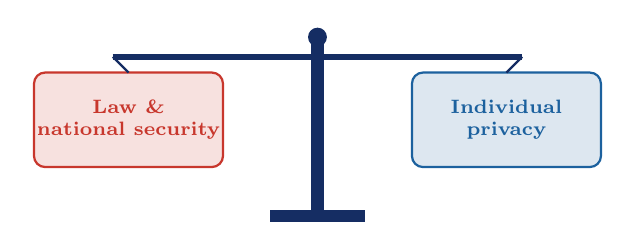
\begin{tikzpicture}
        \draw[navy,line width=2pt] (-2.6,0.8) -- (2.6,0.8);
        \fill[navy] (-0.08,-1.2) rectangle (0.08,1.0);
        \fill[navy] (-0.6,-1.3) rectangle (0.6,-1.15);
        \fill[navy] (0,1.05) circle (0.12);
        \fill[brick!15,draw=brick,thick,rounded corners] (-3.6,-0.6) rectangle (-1.2,0.6);
        \node[font=\scriptsize\bfseries,text=brick,align=center] at (-2.4,0) {Law \&\\national security};
        \fill[ocean!15,draw=ocean,thick,rounded corners] (1.2,-0.6) rectangle (3.6,0.6);
        \node[font=\scriptsize\bfseries,text=ocean,align=center] at (2.4,0) {Individual\\privacy};
        \draw[navy,thick] (-2.6,0.8) -- (-2.4,0.6) (2.6,0.8) -- (2.4,0.6);
      \end{tikzpicture}
    \end{column}
    \begin{column}{0.48\textwidth}
      \begin{itemize}\small\setlength{\itemsep}{4pt}
        \item Court-authorized \textbf{line tapping} helps bring criminals to justice and deters unlawful use of networks
        \item Widespread public-key cryptography may be a \textbf{boost for criminals and terrorists}
        \item Many bills propose that a government agency should be able to obtain the \textbf{clear text} of any communication, under law
      \end{itemize}
      \begin{block}{The challenge}
        \small Build a cryptosystem that \textbf{protects privacy} but still allows \textbf{court-authorized wiretaps}.
      \end{block}
    \end{column}
  \end{columns}
\end{frame}

% ------------------------------------------------------------
\begin{frame}{Two Unpopular Options}
  \centering
  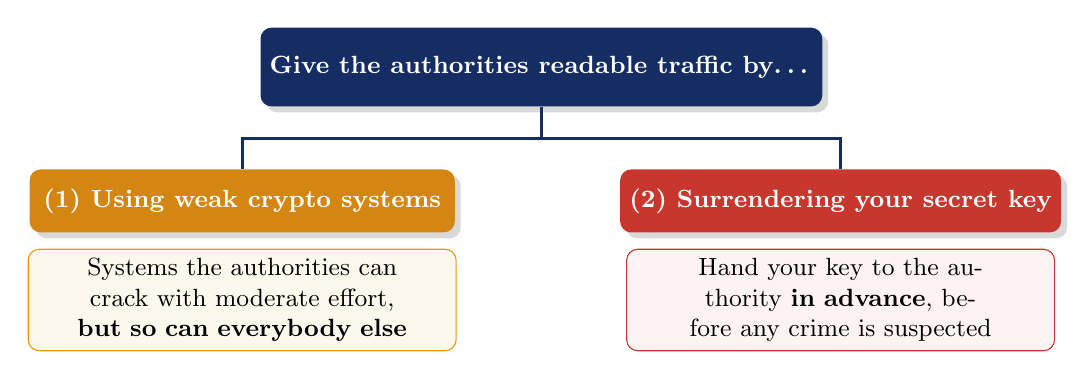
\begin{tikzpicture}
    \node[solid box=navy,minimum width=60mm,minimum height=10mm] (t) at (0,0) {Give the authorities readable traffic by\dots};
    \node[solid box=amber!90!black,minimum width=54mm] (a) at (-3.8,-1.7) {(1) Using weak crypto systems};
    \node[solid box=brick,minimum width=54mm] (b) at (3.8,-1.7) {(2) Surrendering your secret key};
    \draw[navy,very thick] (t.south) -- ++(0,-0.4) -| (a.north);
    \draw[navy,very thick] (t.south) -- ++(0,-0.4) -| (b.north);
    \node[draw=amber,fill=amber!8,rounded corners,text width=52mm,font=\small,anchor=north,align=center] at ([yshift=-2mm]a.south)
      {Systems the authorities can crack with moderate effort, \textbf{but so can everybody else}};
    \node[draw=brick,fill=brick!6,rounded corners,text width=52mm,font=\small,anchor=north,align=center] at ([yshift=-2mm]b.south)
      {Hand your key to the authority \textbf{in advance}, before any crime is suspected};
  \end{tikzpicture}
  \vspace{4mm}
  \begin{alertblock}{Public reaction}
    \small Both alternatives alarmed many citizens, who felt that \textbf{privacy should come before} national security and law enforcement.
  \end{alertblock}
\end{frame}

% ------------------------------------------------------------
\begin{frame}{What Is Key Escrow?}
  \begin{columns}[c]
    \begin{column}{0.5\textwidth}
      \centering
      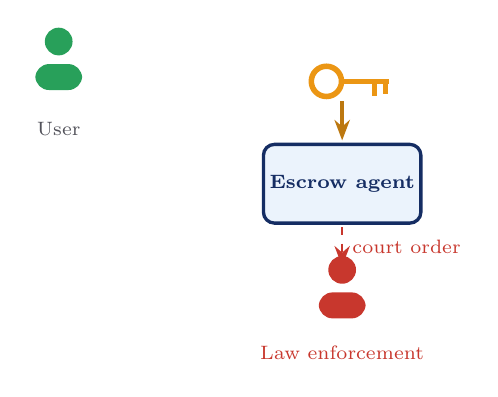
\begin{tikzpicture}
        \pic[scale=1.1] at (0,0.2) {person=leaf}; \node[tag] at (0,-0.4) {User};
        \pic[scale=1.6] at (3.4,0.2) {key=amber};
        \draw[navy,very thick,fill=sky,rounded corners] (2.6,-1.6) rectangle (4.6,-0.6);
        \node[font=\scriptsize\bfseries,text=navy] at (3.6,-1.1) {Escrow agent};
        \draw[->,amber!80!black,very thick] (3.6,-0.05) -- (3.6,-0.55);
        \pic[scale=1.1] at (3.6,-2.7) {person=brick}; \node[tag,text=brick] at (3.6,-3.25) {Law enforcement};
        \draw[->,brick,thick,dashed] (3.6,-1.65) -- node[right,font=\scriptsize]{court order} (3.6,-2.15);
      \end{tikzpicture}
    \end{column}
    \begin{column}{0.48\textwidth}
      \begin{block}{Idea}
        \small A copy of the decryption key (or its pieces) is held in \textbf{escrow} by trusted agents, and released \textbf{only under a court order}.
      \end{block}
      \begin{itemize}\small\setlength{\itemsep}{3pt}
        \item The heart of the US government's \textbf{Clipper} program
        \item Formalized as the \textbf{Escrowed Encryption Standard (EES)}
        \item ``Escrow'' = held by a third party until a condition is met
      \end{itemize}
    \end{column}
  \end{columns}
\end{frame}

% ------------------------------------------------------------
\begin{frame}{The EES Chip and Its Split Key}
  \centering
  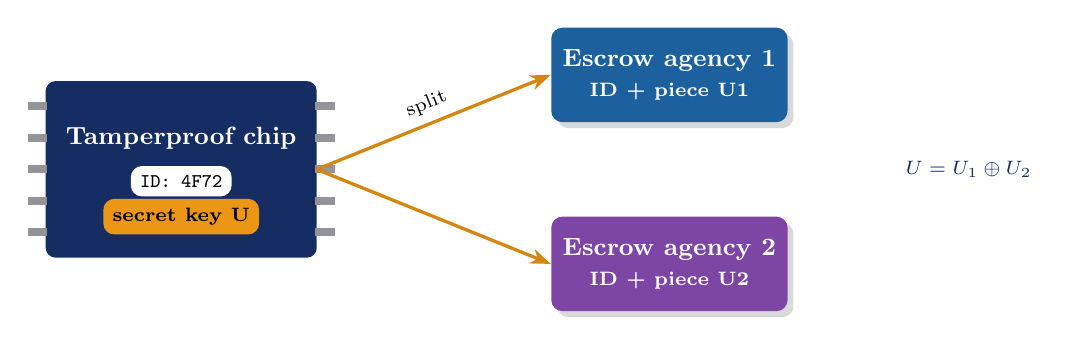
\begin{tikzpicture}
    \node[draw=navy,very thick,fill=navy,rounded corners=3pt,minimum width=34mm,minimum height=22mm] (chip) at (0,0) {};
    \foreach \y in {-0.8,-0.4,0,0.4,0.8}{\fill[ink!50] (-1.95,\y-0.05) rectangle (-1.7,\y+0.05); \fill[ink!50] (1.7,\y-0.05) rectangle (1.95,\y+0.05);}
    \node[white,font=\small\bfseries,align=center] at (0,0.4) {Tamperproof chip};
    \node[fill=white,font=\scriptsize\ttfamily,rounded corners] at (0,-0.15) {ID: 4F72};
    \node[fill=amber,font=\scriptsize\bfseries,rounded corners] at (0,-0.6) {secret key U};
    \node[solid box=ocean,minimum width=30mm,minimum height=12mm] (e1) at (6.2,1.2) {Escrow agency 1\\\scriptsize ID + piece U1};
    \node[solid box=grape,minimum width=30mm,minimum height=12mm] (e2) at (6.2,-1.2) {Escrow agency 2\\\scriptsize ID + piece U2};
    \draw[flow=amber!90!black] (chip.east) -- node[above,font=\scriptsize,sloped]{split} (e1.west);
    \draw[flow=amber!90!black] (chip.east) -- (e2.west);
    \node[font=\scriptsize,text=navy] at (10.0,0) {$U = U_1 \oplus U_2$};
  \end{tikzpicture}
  \vspace{3mm}
  \begin{itemize}\small
    \item EES gets its security from \textbf{tamperproof hardware}
    \item Each chip has a \textbf{unique ID number} and a \textbf{secret key}
    \item The key is split into \textbf{two pieces}, stored with the ID by \textbf{two different escrow agencies}: neither piece alone reveals anything
  \end{itemize}
\end{frame}

% ------------------------------------------------------------
\begin{frame}{How an EES Chip Sends Data}
  \centering
  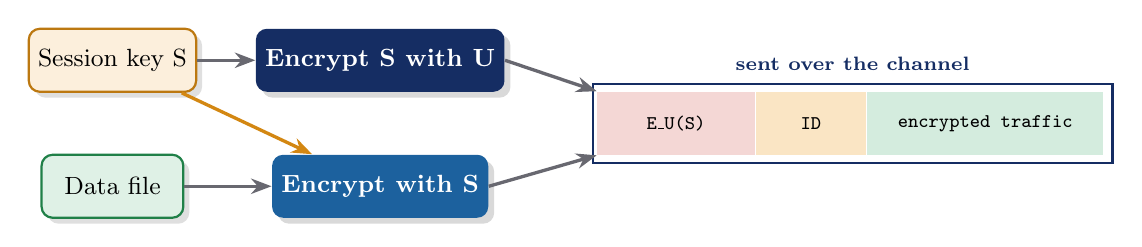
\begin{tikzpicture}
    \node[box=leaf,minimum width=18mm] (d) at (0,0) {Data file};
    \node[box=amber,minimum width=18mm] (k) at (0,1.6) {Session key S};
    \node[solid box=ocean,minimum width=22mm] (e1) at (3.4,0) {Encrypt with S};
    \node[solid box=navy,minimum width=22mm] (e2) at (3.4,1.6) {Encrypt S with U};
    \draw[flow] (d) -- (e1); \draw[flow] (k) -- (e2); \draw[flow=amber!90!black] (k) -- (e1);
    \node[draw=navy,thick,fill=white,minimum width=66mm,minimum height=10mm] (pkt) at (9.4,0.8) {};
    \node[fill=brick!20,font=\scriptsize\ttfamily,minimum width=20mm,minimum height=8mm,anchor=west] (p1) at (6.15,0.8) {E\_U(S)};
    \node[fill=amber!25,font=\scriptsize\ttfamily,minimum width=14mm,minimum height=8mm,anchor=west] (p2) at (p1.east) {ID};
    \node[fill=leaf!20,font=\scriptsize\ttfamily,minimum width=30mm,minimum height=8mm,anchor=west] (p3) at (p2.east) {encrypted traffic};
    \draw[flow] (e2.east) -- (p1.north west);
    \draw[flow] (e1.east) -- (p1.south west);
    \node[font=\scriptsize\bfseries,text=navy] at (9.4,1.55) {sent over the channel};
  \end{tikzpicture}
  \vspace{4mm}
  \begin{block}{Every time the chip encrypts}
    \small It first encrypts the \textbf{session key} with its unique secret key, then sends this encrypted session key and its \textbf{ID number} along with the encrypted traffic.
  \end{block}
\end{frame}

% ------------------------------------------------------------
\begin{frame}{How Law Enforcement Decrypts}
  \centering
  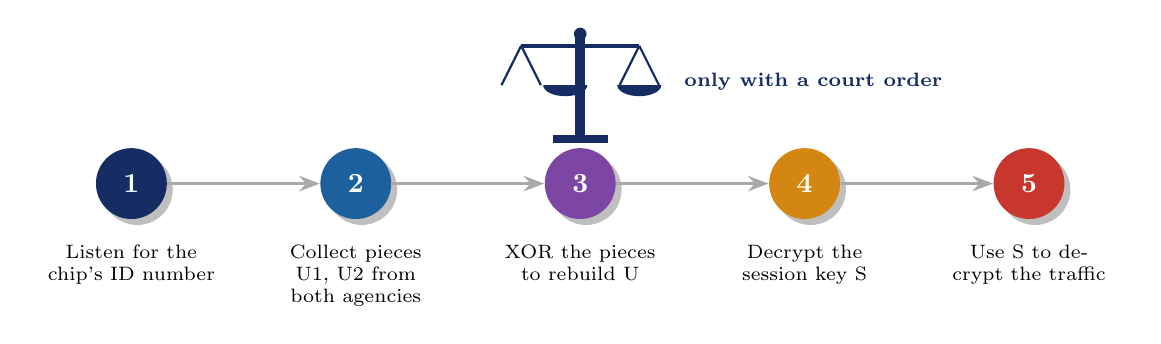
\begin{tikzpicture}
    \foreach \t/\c [count=\i from 0] in {Listen for the chip's ID number/navy,Collect pieces U1\comma{} U2 from both agencies/ocean,XOR the pieces to rebuild U/grape,Decrypt the session key S/amber!90!black,Use S to decrypt the traffic/brick}{
      \node[circle,fill=\c,text=white,font=\bfseries,minimum size=9mm,drop shadow] (c\i) at (\i*2.85,0) {\the\numexpr\i+1\relax};
      \node[font=\scriptsize,text width=24mm,align=center,below=2mm of c\i] {\t};
    }
    \foreach \i [evaluate=\i as \j using int(\i+1)] in {0,1,2,3} \draw[flow=ink!40] (c\i) -- (c\j);
    \pic[scale=1] at (5.7,1.3) {scales=navy};
    \node[font=\scriptsize\bfseries,text=navy,anchor=west] at (6.9,1.3) {only with a court order};
  \end{tikzpicture}
  \vspace{4mm}
  \begin{exampleblock}{The point}
    \small Without the court-ordered help of \textbf{both} escrow agencies, the traffic stays private, but with it, a lawful wiretap is possible.
  \end{exampleblock}
\end{frame}

% ------------------------------------------------------------
\begin{frame}{Secret Splitting with XOR}
  \begin{columns}[c]
    \begin{column}{0.55\textwidth}
      \centering
      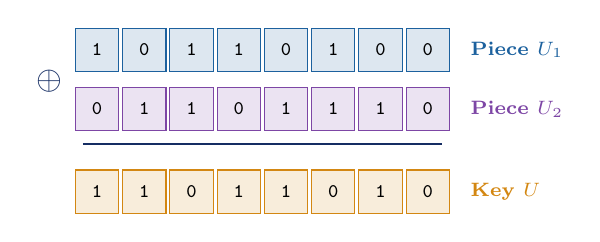
\begin{tikzpicture}[x=6mm]
        \foreach \row/\lab/\bits/\c in {0/Piece $U_1$/{1,0,1,1,0,1,0,0}/ocean,1/Piece $U_2$/{0,1,1,0,1,1,1,0}/grape,2.4/Key $U$/{1,1,0,1,1,0,1,0}/amber!90!black}{
          \node[anchor=west,font=\scriptsize\bfseries,text=\c] at (7.7,-\row*0.75) {\lab};
          \foreach \b [count=\k from 0] in \bits
            \node[draw=\c,fill=\c!15,minimum size=5.5mm,font=\scriptsize\ttfamily] at (\k,-\row*0.75) {\b};
        }
        \draw[navy,thick] (-0.3,-1.2) -- (7.3,-1.2);
        \node[font=\large\bfseries,text=navy] at (-1.0,-0.4) {$\oplus$};
      \end{tikzpicture}
    \end{column}
    \begin{column}{0.43\textwidth}
      \begin{itemize}\small\setlength{\itemsep}{4pt}
        \item XOR rule: \textbf{same bits give 0}, different bits give 1
        \item $U_1$ alone looks completely \textbf{random}; so does $U_2$
        \item Only $U_1 \oplus U_2$ gives back the real key $U$
      \end{itemize}
      \begin{block}{So}
        \small One agency, or one thief who robs one agency, learns \textbf{nothing} about the key.
      \end{block}
    \end{column}
  \end{columns}
\end{frame}

% ------------------------------------------------------------
\begin{frame}{Escrow with $n$ Trustees}
  \begin{columns}[c]
    \begin{column}{0.5\textwidth}
      \centering
      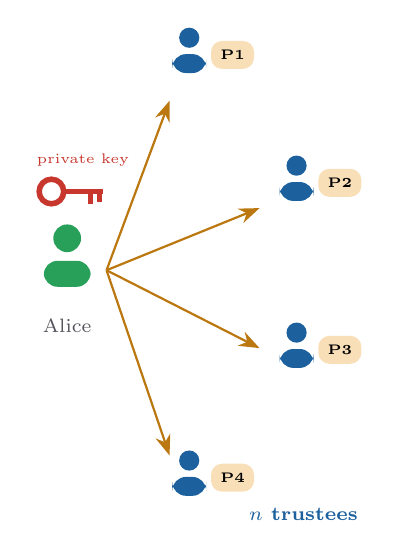
\begin{tikzpicture}
        \pic[scale=1.1] at (0,0) {person=leaf}; \node[tag] at (0,-0.6) {Alice};
        \pic[scale=1.3] at (-0.2,1.1) {key=brick};
        \node[font=\tiny,text=brick] at (0.2,1.5) {private key};
        \foreach \a [count=\i] in {60,20,-20,-60}{
          \pic[scale=0.8] at ($(0,0)+(\a:3.1)$) {person=ocean};
          \node[font=\tiny\bfseries,fill=amber!30,rounded corners] at ($(0,0)+(\a:3.1)+(0.55,0.15)$) {P\i};
          \draw[->,amber!80!black,thick] (0.5,0.1) -- ($(0,0)+(\a:2.6)$);
        }
        \node[font=\scriptsize\bfseries,text=ocean] at (3.0,-3.0) {$n$ trustees};
      \end{tikzpicture}
    \end{column}
    \begin{column}{0.48\textwidth}
      \begin{itemize}\small\setlength{\itemsep}{4pt}
        \item Alice's \textbf{private key} is broken into pieces and given to different \textbf{trustees}
        \item Like a \textbf{secret sharing} scheme: together, the authorities can rebuild the key
        \item Each trustee can \textbf{verify} their piece is valid without rebuilding the key
        \item Alice cannot cheat by sending a random-bit string
      \end{itemize}
      \begin{alertblock}{Hard to abuse}
        \small To steal Alice's key, Mallory must corrupt \textbf{all $n$} trustees.
      \end{alertblock}
    \end{column}
  \end{columns}
\end{frame}

% ------------------------------------------------------------
\begin{frame}{The Trustee Protocol}
  \centering
  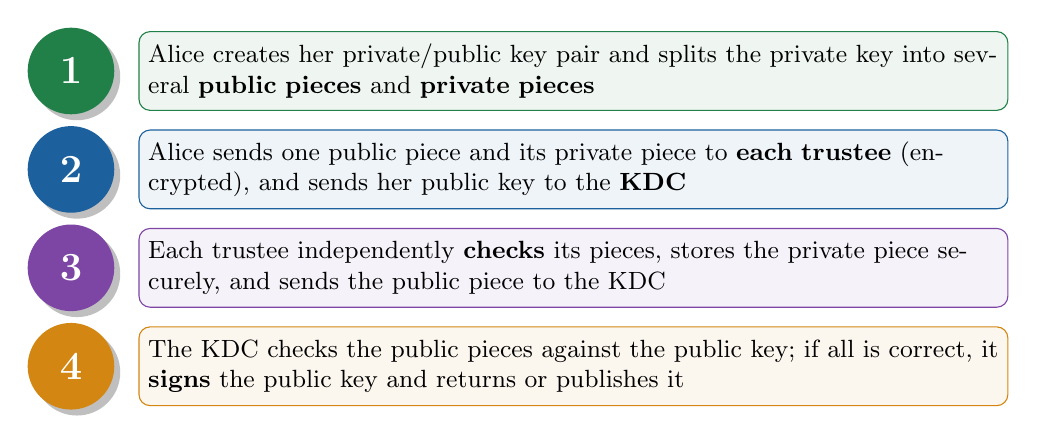
\begin{tikzpicture}
    \foreach \t/\c [count=\i] in {
      Alice creates her private\slash public key pair and splits the private key into several \textbf{public pieces} and \textbf{private pieces}/leaf!80!black,
      Alice sends one public piece and its private piece to \textbf{each trustee} (encrypted)\comma{} and sends her public key to the \textbf{KDC}/ocean,
      Each trustee independently \textbf{checks} its pieces\comma{} stores the private piece securely\comma{} and sends the public piece to the KDC/grape,
      The KDC checks the public pieces against the public key; if all is correct\comma{} it \textbf{signs} the public key and returns or publishes it/amber!90!black}
    {
      \node[circle,fill=\c,text=white,font=\Large\bfseries,minimum size=11mm,drop shadow] (c\i) at (0,-\i*1.25) {\i};
      \node[draw=\c,fill=\c!7,rounded corners=4pt,anchor=west,text width=108mm,minimum height=10mm,font=\small] at ([xshift=3mm]c\i.east) {\t};
    }
  \end{tikzpicture}
  \vspace{2mm}

  {\small KDC = Key Distribution Centre.}
\end{frame}

% ------------------------------------------------------------
\begin{frame}{When the Court Orders a Wiretap}
  \centering
  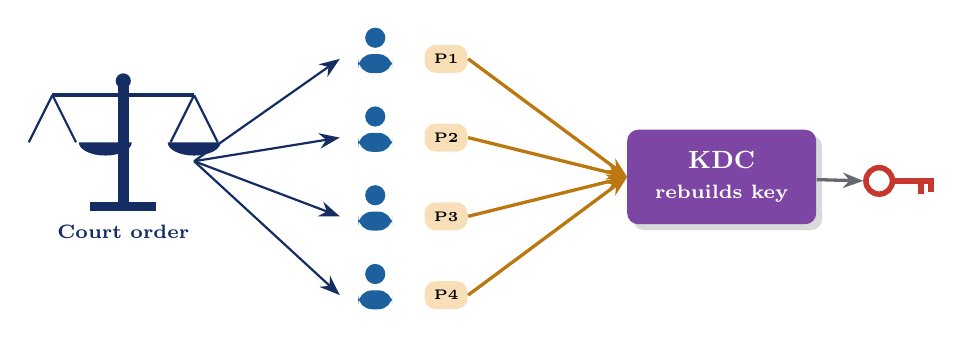
\begin{tikzpicture}
    \pic[scale=1.2] at (0,0.6) {scales=navy};
    \node[font=\scriptsize\bfseries,text=navy] at (0,-0.6) {Court order};
    \foreach \y [count=\i] in {1.5,0.5,-0.5,-1.5}{
      \pic[scale=0.8] at (3.2,\y) {person=ocean};
      \node[fill=amber!30,font=\tiny\bfseries,rounded corners] (p\i) at (4.1,\y+0.1) {P\i};
      \draw[->,navy,thick] (0.9,0.3) -- (2.75,\y+0.1);
      \draw[->,amber!80!black,very thick] (p\i.east) -- (6.4,0.1);
    }
    \node[solid box=grape,minimum width=24mm,minimum height=12mm] (kdc) at (7.6,0.1) {KDC\\\scriptsize rebuilds key};
    \pic[scale=1.4] at (9.6,0.05) {key=brick};
    \draw[flow] (kdc) -- (9.4,0.05);
  \end{tikzpicture}
  \vspace{3mm}
  \begin{columns}[T]
    \begin{column}{0.5\textwidth}
      \begin{block}{After the order}
        \small \textbf{Each} trustee surrenders its piece to the KDC, which reconstructs the private key and can wiretap Alice.
      \end{block}
    \end{column}
    \begin{column}{0.46\textwidth}
      \begin{alertblock}{Before the order}
        \small Neither the KDC nor any single trustee can rebuild the key: \textbf{all trustees} are required.
      \end{alertblock}
    \end{column}
  \end{columns}
\end{frame}

% ------------------------------------------------------------
\begin{frame}{The Politics: What Does the User Gain?}
  \begin{columns}[c]
    \begin{column}{0.48\textwidth}
      \centering
      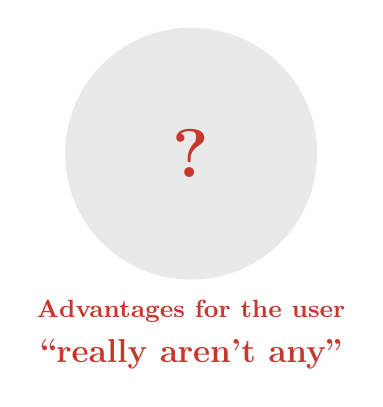
\begin{tikzpicture}
        \fill[ink!10] (0,0) circle (1.6);
        \node[font=\fontsize{40}{40}\selectfont\bfseries,text=brick] at (0,0) {?};
        \node[font=\small\bfseries,text=brick] at (0,-2.0) {Advantages for the user};
        \node[font=\large\bfseries,text=brick] at (0,-2.55) {``really aren't any''};
      \end{tikzpicture}
    \end{column}
    \begin{column}{0.5\textwidth}
      {\small Several \textbf{commercial} key-escrow proposals exist besides the government's. But the user gains nothing he could not provide himself:}
      \begin{itemize}\small\setlength{\itemsep}{3pt}
        \item He can already \textbf{back up his own keys}
        \item Escrow guarantees the \textbf{police can eavesdrop} on his conversations and read his files, even though encrypted
        \item It guarantees the \textbf{NSA can eavesdrop} on international calls, \textbf{without a warrant}
        \item Perhaps he may use crypto in countries that would ban it, the \textbf{only advantage}
      \end{itemize}
    \end{column}
  \end{columns}
\end{frame}

% ------------------------------------------------------------
\begin{frame}{The Politics: Considerable Disadvantages}
  \centering
  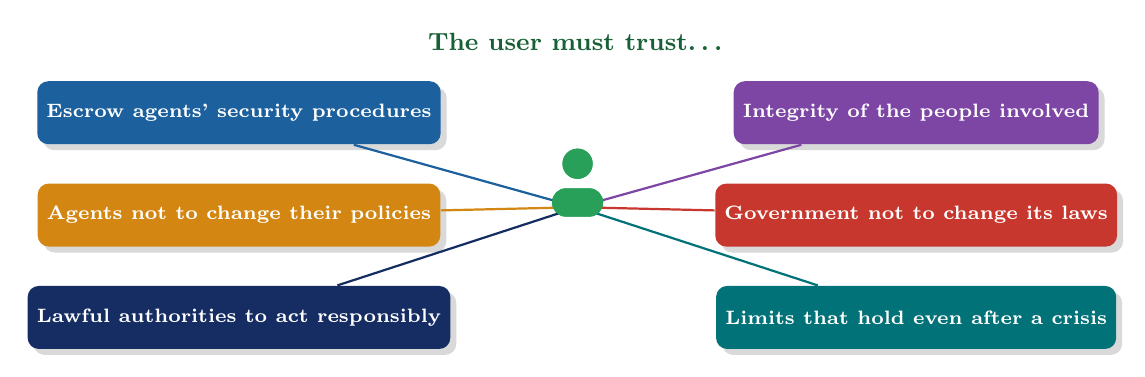
\begin{tikzpicture}
    \pic[scale=1.2] at (0,0.1) {person=leaf};
    \node[font=\small\bfseries,text=leaf!60!black,fill=white,inner sep=2pt] at (0,2.2) {The user must trust\dots};
    \foreach \x/\y/\t/\c in {-4.3/1.3/Escrow agents' security procedures/ocean,4.3/1.3/Integrity of the people involved/grape,-4.3/0/Agents not to change their policies/amber!90!black,4.3/0/Government not to change its laws/brick,-4.3/-1.3/Lawful authorities to act responsibly/navy,4.3/-1.3/Limits that hold even after a crisis/aqua!80!black}{
      \node[solid box=\c,minimum width=42mm,minimum height=8mm,font=\scriptsize\bfseries] (s) at (\x,\y) {\t};
      \draw[\c,thick] (0,0.1) -- (s);
    }
    \pic[scale=1.2] at (0,0.1) {person=leaf};
  \end{tikzpicture}
  \vspace{4mm}
  \begin{alertblock}{A thought experiment}
    \small Imagine a major terrorist attack in New York: what sorts of limits on the police would be \textbf{thrown aside} in the aftermath?
  \end{alertblock}
\end{frame}

% ------------------------------------------------------------
\begin{frame}{Where Escrow Leads: Legal Pressure}
  \begin{columns}[c]
    \begin{column}{0.5\textwidth}
      \centering
      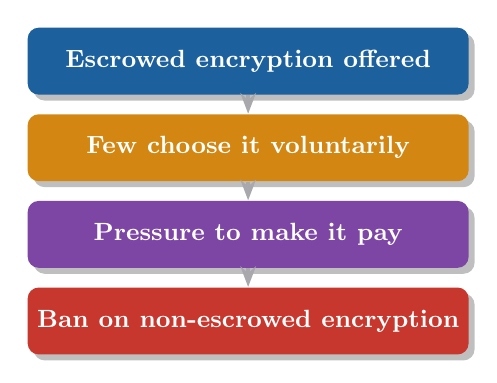
\begin{tikzpicture}
        \foreach \t/\c [count=\i from 0] in {Escrowed encryption offered/ocean,Few choose it voluntarily/amber!90!black,Pressure to make it pay/grape,Ban on non-escrowed encryption/brick}{
          \node[fill=\c,text=white,rounded corners=4pt,font=\small\bfseries,minimum width=56mm,minimum height=8.5mm,drop shadow] (s\i) at (0,-\i*1.1) {\t};
        }
        \foreach \i [evaluate=\i as \j using int(\i+1)] in {0,1,2} \draw[flow=ink!40] (s\i) -- (s\j);
      \end{tikzpicture}
    \end{column}
    \begin{column}{0.48\textwidth}
      \begin{itemize}\small\setlength{\itemsep}{4pt}
        \item Escrow is hard to imagine working \textbf{without legal pressure}
        \item The obvious next step: \textbf{ban non-escrowed} encryption, the only way to force sophisticated criminals to use it
      \end{itemize}
      \begin{alertblock}{Open questions}
        \small How hard would such a ban be? How would it affect cryptography as an \textbf{academic discipline}? Would a researcher need a \textbf{special licence} to study non-escrowed algorithms?
      \end{alertblock}
    \end{column}
  \end{columns}
\end{frame}

% ============================================================
\setcounter{section}{7}
\section{Legal Issues}
% ============================================================

\begin{frame}{The OSI Standard for Security Model}
  \begin{columns}[c]
    \begin{column}{0.45\textwidth}
      \centering
      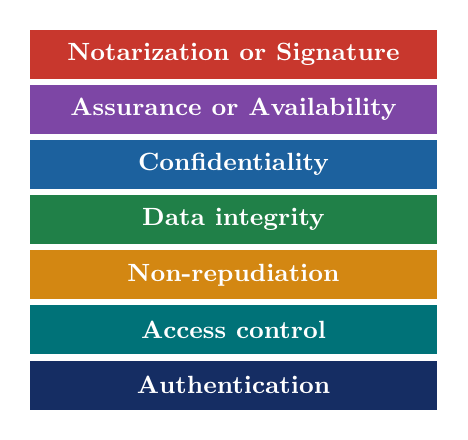
\begin{tikzpicture}
        \foreach \t/\c [count=\i] in {Notarization or Signature/brick,Assurance or Availability/grape,Confidentiality/ocean,Data integrity/leaf!80!black,Non-repudiation/amber!90!black,Access control/aqua!80!black,Authentication/navy}
          \node[layer=\c,minimum width=52mm,minimum height=6.5mm] at (0,-\i*0.7) {\t};
      \end{tikzpicture}
    \end{column}
    \begin{column}{0.53\textwidth}
      \begin{itemize}\small\setlength{\itemsep}{5pt}
        \item You know the \textbf{OSI network model}: seven layers from physical to application
        \item A much less known standard on similar lines is the \textbf{OSI standard for Security Model}
        \item It also defines \textbf{seven layers of security}, shown on the left
      \end{itemize}
      \begin{block}{Link to Module 2}
        \small These match the \textbf{security services} we studied: authentication, access control, integrity, confidentiality, availability and non-repudiation.
      \end{block}
    \end{column}
  \end{columns}
\end{frame}

% ------------------------------------------------------------
\begin{frame}{Ethical Issues: Privacy vs.\ the Greater Good}
  \begin{columns}[c]
    \begin{column}{0.5\textwidth}
      \centering
      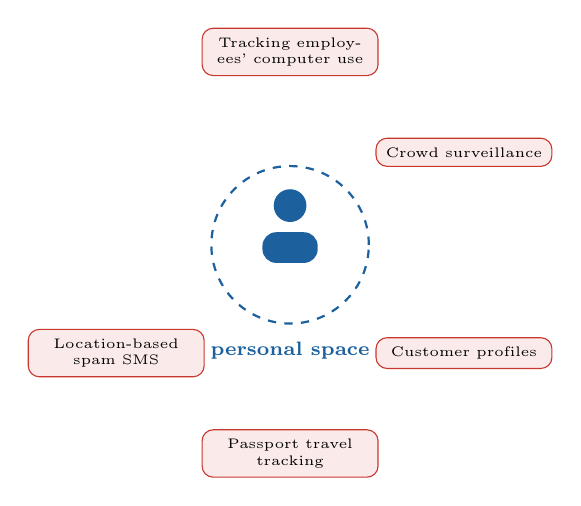
\begin{tikzpicture}
        \pic[scale=1.3] at (0,0) {person=ocean};
        \draw[ocean,dashed,thick] (0,0.1) circle (1.0);
        \node[font=\scriptsize\bfseries,text=ocean] at (0,-1.25) {personal space};
        \foreach \a/\t in {90/Tracking employees' computer use,30/Crowd surveillance,-30/Customer profiles,-90/Passport travel tracking,210/Location-based spam SMS}{
          \node[fill=brick!10,draw=brick,rounded corners,font=\tiny,text width=20mm,align=center] (e\a) at (\a:2.55) {\t};
        }
      \end{tikzpicture}
    \end{column}
    \begin{column}{0.48\textwidth}
      \begin{itemize}\small\setlength{\itemsep}{4pt}
        \item Many ethical and legal issues are about the \textbf{individual's right to privacy} versus the \textbf{greater good} of a company or society
        \item Examples are shown around the person on the left
      \end{itemize}
      \begin{block}{Key concept}
        \small To resolve such issues, ask: what is the person's \textbf{expectation of privacy}?
      \end{block}
    \end{column}
  \end{columns}
\end{frame}

% ------------------------------------------------------------
\begin{frame}{Four Ethical Categories: PAPA}
  \centering
  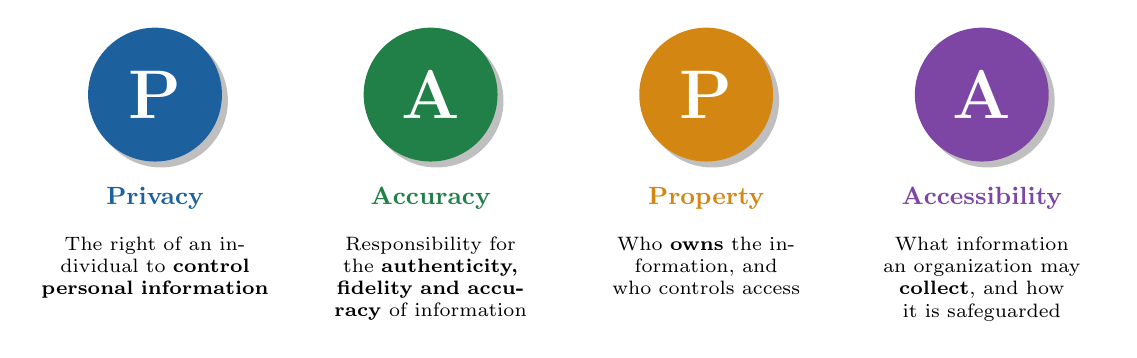
\begin{tikzpicture}
    \foreach \x/\c/\l/\t/\d in {
      0/ocean/P/Privacy/The right of an individual to \textbf{control personal information},
      3.5/leaf!80!black/A/Accuracy/Responsibility for the \textbf{authenticity\comma{} fidelity and accuracy} of information,
      7/amber!90!black/P/Property/Who \textbf{owns} the information\comma{} and who controls access,
      10.5/grape/A/Accessibility/What information an organization may \textbf{collect}\comma{} and how it is safeguarded}
    {
      \node[circle,fill=\c,text=white,font=\fontsize{24}{24}\selectfont\bfseries,minimum size=17mm,drop shadow] (c) at (\x,0) {\l};
      \node[font=\small\bfseries,text=\c,below=2mm of c] (t) {\t};
      \node[font=\scriptsize,text width=30mm,align=center,below=1mm of t] {\d};
    }
  \end{tikzpicture}
  \vspace{4mm}

  {\small Classically, ethical issues in security systems fall into these four categories. Remember them as \textbf{PAPA}.}
\end{frame}

% ------------------------------------------------------------
\begin{frame}{What Is Privacy?}
  \begin{columns}[c]
    \begin{column}{0.45\textwidth}
      \centering
      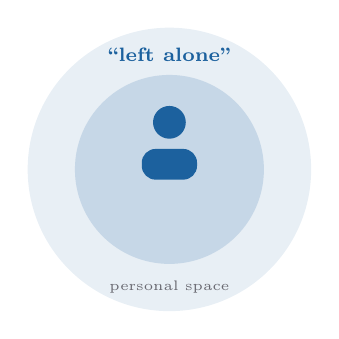
\begin{tikzpicture}
        \fill[ocean!10] (0,0) circle (1.8);
        \fill[ocean!25] (0,0) circle (1.2);
        \pic[scale=1.3] at (0,0) {person=ocean};
        \node[font=\scriptsize\bfseries,text=ocean] at (0,1.45) {``left alone''};
        \node[font=\tiny,text=ink!70] at (0,-1.5) {personal space};
      \end{tikzpicture}
    \end{column}
    \begin{column}{0.53\textwidth}
      \begin{block}{Definition}
        \small Privacy is the protection of \textbf{personal or sensitive information}: the desire to be \textbf{left alone}, as an extension of our personal space.
      \end{block}
      \begin{itemize}\small\setlength{\itemsep}{4pt}
        \item It may or may not be \textbf{supported by local laws}
        \item Privacy is \textbf{subjective}: different people have different ideas of it
        \item People trade different amounts of privacy for \textbf{safety or convenience}
      \end{itemize}
    \end{column}
  \end{columns}
\end{frame}

% ------------------------------------------------------------
\begin{frame}{A Hierarchy of Regulatory Bodies}
  \centering
  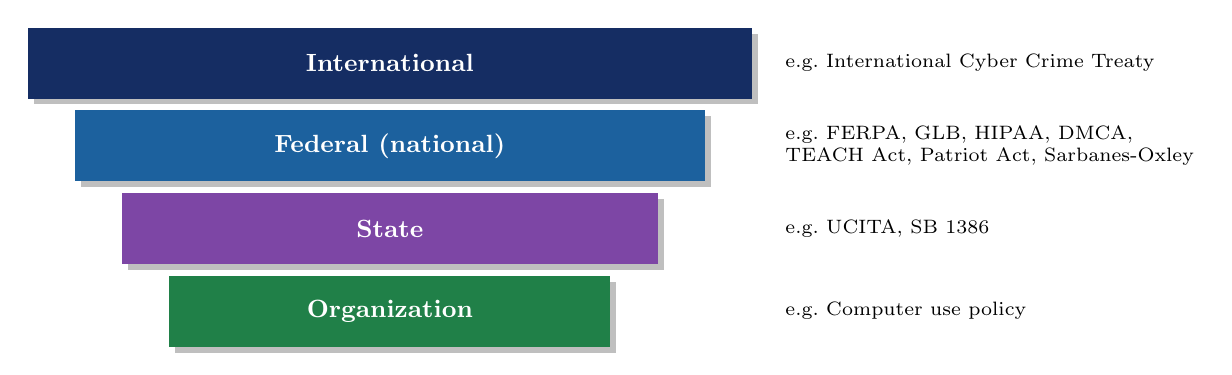
\begin{tikzpicture}
    \foreach \t/\e/\c/\w [count=\i from 0] in {
      International/International Cyber Crime Treaty/navy/92,
      Federal (national)/FERPA\comma{} GLB\comma{} HIPAA\comma{} DMCA\comma{} TEACH Act\comma{} Patriot Act\comma{} Sarbanes-Oxley/ocean/80,
      State/UCITA\comma{} SB 1386/grape/68,
      Organization/Computer use policy/leaf!80!black/56}
    {
      \node[fill=\c,text=white,font=\small\bfseries,minimum width=\w mm,minimum height=9mm,drop shadow] (l\i) at (0,-\i*1.05) {\t};
      \node[anchor=west,font=\scriptsize,text width=52mm] at (4.9,-\i*1.05) {e.g.\ \e};
    }
  \end{tikzpicture}
  \vspace{3mm}
  \begin{block}{Remember}
    \small Legal issues are governed by a \textbf{hierarchy}: an organization's policy must obey state law, which must obey national law, which must fit international treaties.
  \end{block}
\end{frame}

% ------------------------------------------------------------
\begin{frame}{Are Digital Signatures Real Signatures?}
  \centering
  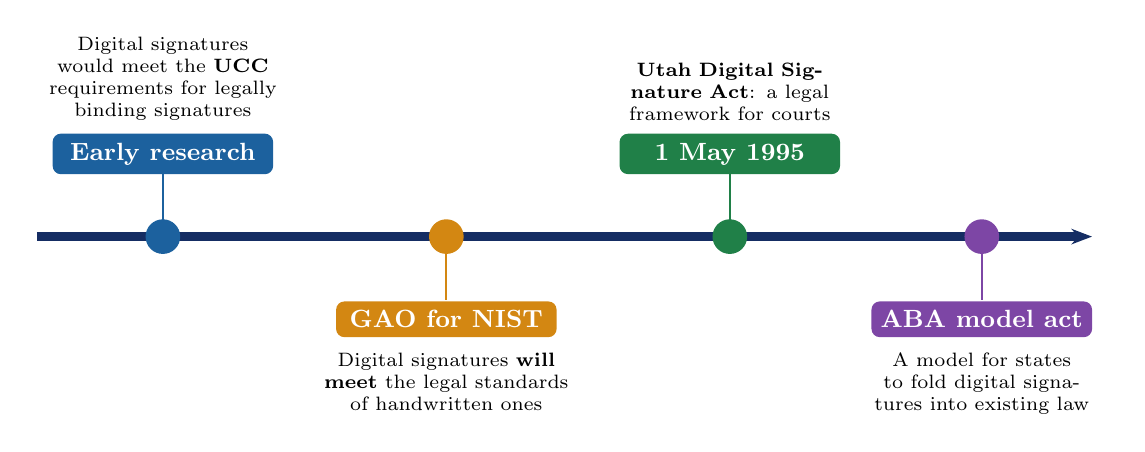
\begin{tikzpicture}
    \draw[navy,line width=3pt,->] (0,0) -- (13.4,0);
    \foreach \x/\c/\y/\t/\d in {
      1.6/ocean/1/Early research/Digital signatures would meet the \textbf{UCC} requirements for legally binding signatures,
      5.2/amber!90!black/-1/GAO for NIST/Digital signatures \textbf{will meet} the legal standards of handwritten ones,
      8.8/leaf!80!black/1/1 May 1995/\textbf{Utah Digital Signature Act}: a legal framework for courts,
      12.0/grape/-1/ABA model act/A model for states to fold digital signatures into existing law}
    {
      \fill[\c] (\x,0) circle (2.2mm);
      \draw[\c,thick] (\x,0) -- (\x,\y*0.8);
      \node[fill=\c,text=white,rounded corners=3pt,font=\small\bfseries,minimum width=28mm] at (\x,\y*1.05) {\t};
      \ifnum\y>0 \node[font=\scriptsize,text width=32mm,align=center,anchor=south] at (\x,1.35) {\d};
      \else \node[font=\scriptsize,text width=32mm,align=center,anchor=north] at (\x,-1.35) {\d};\fi
    }
  \end{tikzpicture}
  \vspace{3mm}

  {\small UCC = Uniform Commercial Code; GAO = General Accounting Office; ABA = American Bar Association.}
\end{frame}

% ------------------------------------------------------------
\begin{frame}{The ABA Model Act and Its Limits}
  \begin{columns}[T]
    \begin{column}{0.49\textwidth}
      \begin{block}{The model act includes}
        \small
        \begin{itemize}\setlength{\itemsep}{2pt}
          \item Fitting digital signatures into existing law: UCC, US Federal Reserve rules, contract law, UN conventions on sale of goods and bills of exchange
          \item Responsibilities and obligations of \textbf{certification authorities}
          \item Issues of \textbf{liability}, limits and policies
        \end{itemize}
      \end{block}
    \end{column}
    \begin{column}{0.49\textwidth}
      \begin{alertblock}{Still undefined}
        \small In the US, signature and contract laws are \textbf{state} laws, so the act targets states; a federal act is the eventual goal. The validity of digital signatures had \textbf{not yet been tested in court}.
      \end{alertblock}
      \centering
      
\begin{tikzpicture}
        \foreach \i in {0,...,4} \node[circle,fill=ocean!\the\numexpr 30+\i*15\relax,minimum size=6mm] at (\i*0.8,0) {};
        \node[font=\tiny,text=ink!70] at (1.6,-0.5) {precedent builds up case by case};
      \end{tikzpicture}
    \end{column}
  \end{columns}
\end{frame}

% ------------------------------------------------------------
\begin{frame}{Until Courts Decide: The Paper Contract}
  \centering
  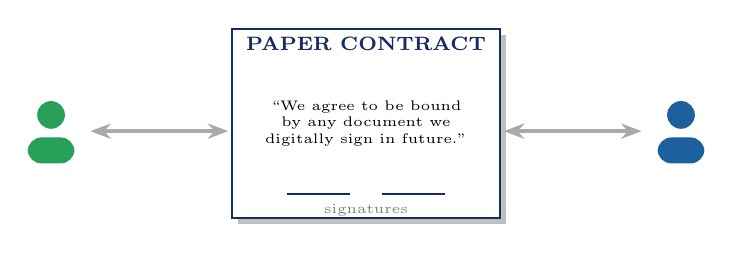
\begin{tikzpicture}
    \pic[scale=1.1] at (0,0) {person=leaf};
    \pic[scale=1.1] at (8,0) {person=ocean};
    \node[draw=navy,thick,fill=white,minimum width=34mm,minimum height=24mm,drop shadow] (pc) at (4,0.4) {};
    \node[font=\scriptsize\bfseries,text=navy,anchor=north] at (pc.north) {PAPER CONTRACT};
    \node[font=\tiny,text width=30mm,align=center] at (4,0.4) {``We agree to be bound by any document we digitally sign in future.''};
    \draw[navy,thick] (3.0,-0.5) -- (3.8,-0.5) (4.2,-0.5) -- (5.0,-0.5);
    \node[font=\tiny,text=ink!60] at (4,-0.7) {signatures};
    \draw[<->,very thick,ink!40] (0.5,0.3) -- (2.25,0.3);
    \draw[<->,very thick,ink!40] (5.75,0.3) -- (7.5,0.3);
  \end{tikzpicture}
  \vspace{3mm}
  \begin{itemize}\small
    \item For digital signatures to have the same authority as handwritten ones, they must first be used, \textbf{challenged in court}, and ruled on, again and again
    \item A body of \textbf{precedent} would then say which methods and key sizes are legally binding; this takes years
    \item Until then: first sign a \textbf{paper contract} agreeing to honour your digital signatures
  \end{itemize}
\end{frame}

% ------------------------------------------------------------
\begin{frame}{Security and Law: Different Speeds}
  \begin{columns}[c]
    \begin{column}{0.5\textwidth}
      \centering
      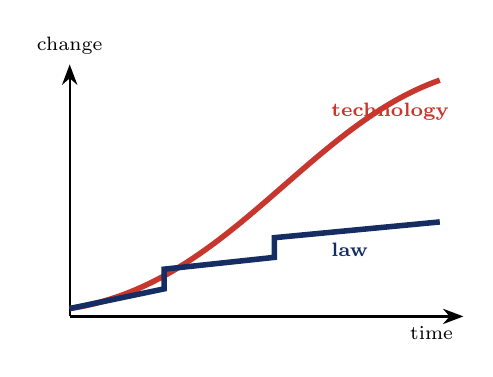
\begin{tikzpicture}
        \draw[->,thick] (0,0) -- (5,0) node[below left,font=\scriptsize]{time};
        \draw[->,thick] (0,0) -- (0,3.2) node[above,font=\scriptsize]{change};
        \draw[brick,line width=2pt] (0,0.1) .. controls (2,0.4) and (3,2.4) .. (4.7,3.0);
        \draw[navy,line width=2pt] (0,0.1) -- (1.2,0.35) -- (1.2,0.6) -- (2.6,0.75) -- (2.6,1.0) -- (4.7,1.2);
        \node[font=\scriptsize\bfseries,text=brick,anchor=west] at (3.2,2.6) {technology};
        \node[font=\scriptsize\bfseries,text=navy,anchor=west] at (3.2,0.85) {law};
      \end{tikzpicture}
    \end{column}
    \begin{column}{0.48\textwidth}
      \begin{itemize}\small\setlength{\itemsep}{3pt}
        \item As security changes our lives, laws enable desired behaviour and prohibit undesired behaviour
        \item But information technology moves \textbf{much faster} than law-making
        \item Sometimes laws are \textbf{too restrictive} (import/export of encryption)
        \item Sometimes \textbf{too slow} (digital signatures)
        \item Sometimes both (privacy laws)
      \end{itemize}
      {\small\textit{You will never satisfy everyone with a law, but it does set the rules of the game.}}
    \end{column}
  \end{columns}
\end{frame}

% ------------------------------------------------------------
\begin{frame}{Regulations in India}
  \begin{columns}[c]
    \begin{column}{0.45\textwidth}
      \centering
      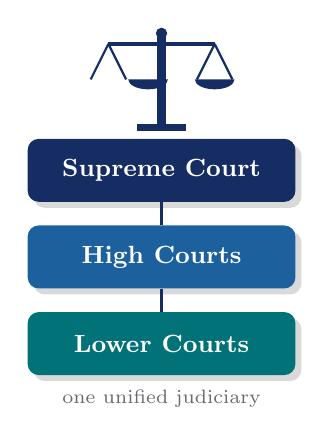
\begin{tikzpicture}
        \pic[scale=0.9] at (0,2.2) {scales=navy};
        \node[solid box=navy,minimum width=34mm] (sc) at (0,1.0) {Supreme Court};
        \node[solid box=ocean,minimum width=34mm] (hc) at (0,-0.1) {High Courts};
        \node[solid box=aqua!80!black,minimum width=34mm] (lc) at (0,-1.2) {Lower Courts};
        \draw[navy,very thick] (sc) -- (hc) -- (lc);
        \node[font=\scriptsize,text=ink!70] at (0,-1.9) {one unified judiciary};
      \end{tikzpicture}
    \end{column}
    \begin{column}{0.53\textwidth}
      \begin{itemize}\small\setlength{\itemsep}{4pt}
        \item India has a detailed legal system based on \textbf{English common law}
        \item Older laws did not cover the \textbf{Internet} and \textbf{offshoring}, which created complex new legal issues
        \item The government responded \textbf{proactively}: first draft of the IT Bill in \textbf{1999}, the \textbf{IT Act} in \textbf{2000}
        \item The \textbf{Copyright Act} covers computer programs
      \end{itemize}
      \begin{alertblock}{No specific data-protection law}
        \small Instead, several \textbf{proxy laws} provide indirect safeguards, as we will see.
      \end{alertblock}
    \end{column}
  \end{columns}
\end{frame}

% ------------------------------------------------------------
\begin{frame}{Information Technology Act, 2000}
  \centering
  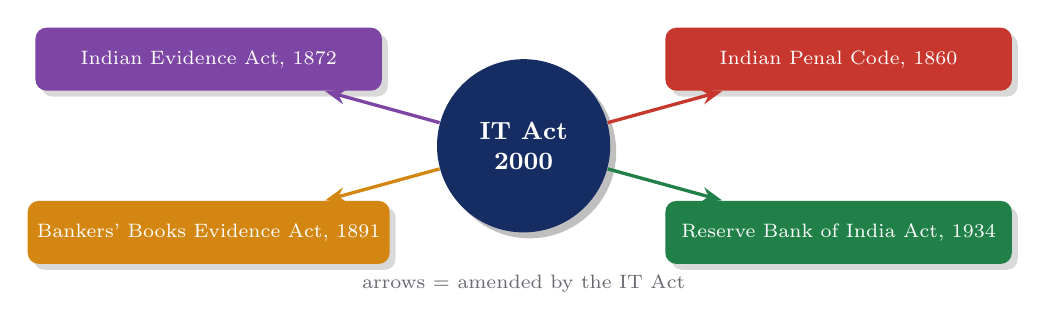
\begin{tikzpicture}
    \node[circle,fill=navy,text=white,font=\small\bfseries,minimum size=22mm,align=center,drop shadow] (it) at (0,0) {IT Act\\2000};
    \foreach \a/\t/\c/\px/\py in {45/Indian Penal Code\comma{} 1860/brick/4.0/1.1,135/Indian Evidence Act\comma{} 1872/grape/-4.0/1.1,225/Bankers' Books Evidence Act\comma{} 1891/amber!90!black/-4.0/-1.1,315/Reserve Bank of India Act\comma{} 1934/leaf!80!black/4.0/-1.1}{
      \node[solid box=\c,minimum width=44mm,font=\scriptsize] (s\a) at (\px,\py) {\t};
      \draw[->,\c,very thick] (it) -- (s\a);
    }
    \node[font=\scriptsize,text=ink!70] at (0,-1.75) {arrows = amended by the IT Act};
  \end{tikzpicture}
  \vspace{2mm}
  \begin{block}{Background}
    \small Passed by both houses of Parliament in \textbf{May 2000}. It covers \textbf{cyber and IT-related laws} in India, and updated older acts with its provisions.
  \end{block}
\end{frame}

% ------------------------------------------------------------
\begin{frame}{IT Act: Section 43}
  \begin{columns}[c]
    \begin{column}{0.48\textwidth}
      \centering
      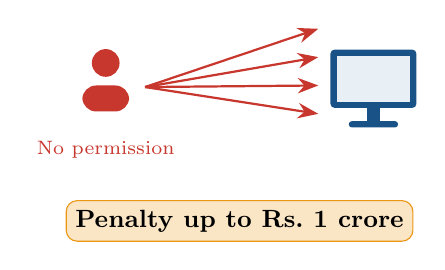
\begin{tikzpicture}
        \pic[scale=1.1] at (0,0) {person=brick}; \node[tag,text=brick] at (0,-0.6) {No permission};
        \pic[scale=1.3] at (3.4,0) {pc=ocean};
        \foreach \t/\y in {accesses/1.4,downloads data/0.8,introduces virus/0.2,denies access/-0.4}{
          \draw[->,brick,thick] (0.5,0.2) -- (2.7,\y*0.6+0.1);
        }
        \node[fill=amber!25,draw=amber,rounded corners,font=\small\bfseries] at (1.7,-1.5) {Penalty up to Rs.\ 1 crore};
      \end{tikzpicture}
    \end{column}
    \begin{column}{0.5\textwidth}
      \begin{block}{Section 43}
        \small If a person, \textbf{without permission} of the person in charge of a computer system:
        \begin{itemize}\setlength{\itemsep}{1pt}
          \item accesses it,
          \item downloads any data,
          \item introduces a virus, or
          \item causes denial of access,
        \end{itemize}
        they are liable for a penalty of up to \textbf{Rs.\ 10 million} (1 crore).
      \end{block}
    \end{column}
  \end{columns}
\end{frame}

% ------------------------------------------------------------
\begin{frame}{IT Act: Sections 65 and 66}
  \begin{columns}[T]
    \begin{column}{0.49\textwidth}
      \centering\textbf{\textcolor{grape}{Section 65: Tampering with Source Code}}\\[2mm]
      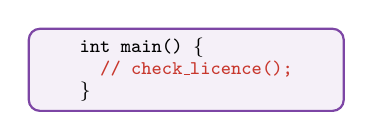
\begin{tikzpicture}
        \node[draw=grape,fill=grape!8,thick,rounded corners,font=\scriptsize\ttfamily,align=left,minimum width=40mm] {int main() \{\\\quad \textcolor{brick}{// check\_licence();}\\\}};
      \end{tikzpicture}\\[2mm]
      {\small Knowingly \textbf{hiding, destroying or altering} computer source code, or getting someone else to.}\\[2mm]
      \tikz\node[fill=grape!15,rounded corners,text width=60mm,align=center,font=\small]{Up to \textbf{3 years} jail, or fine up to \textbf{Rs.\ 2 lakh}, or both};
    \end{column}
    \begin{column}{0.49\textwidth}
      \centering\textbf{\textcolor{brick}{Section 66: Hacking}}\\[2mm]
      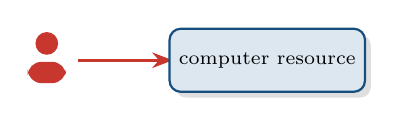
\begin{tikzpicture}
        \pic[scale=0.9] at (0,0) {person=brick};
        \draw[->,brick,very thick] (0.4,0.2) -- (1.6,0.2);
        \node[box=ocean,font=\scriptsize,minimum width=22mm] at (2.8,0.2) {computer resource};
      \end{tikzpicture}\\[2mm]
      {\small With intent to cause \textbf{wrongful loss or damage}, destroying, deleting or altering information, reducing its value or utility, or harming it by any means.}\\[2mm]
      \tikz\node[fill=brick!15,rounded corners,text width=60mm,align=center,font=\small]{Up to \textbf{3 years} jail, or fine up to \textbf{Rs.\ 2 lakh}, or both};
    \end{column}
  \end{columns}
\end{frame}

% ------------------------------------------------------------
\begin{frame}{IT Act: Section 72}
  \begin{columns}[c]
    \begin{column}{0.48\textwidth}
      \centering
      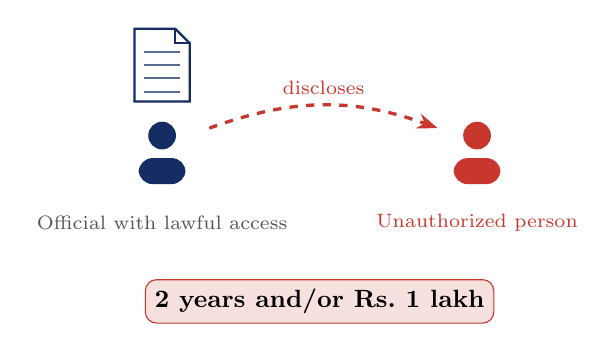
\begin{tikzpicture}
        \pic[scale=1.1] at (0,0) {person=navy}; \node[tag] at (0,-0.6) {Official with lawful access};
        \pic[scale=1.4] at (0,1.4) {doc=navy};
        \pic[scale=1.1] at (4,0) {person=brick}; \node[tag,text=brick] at (4,-0.6) {Unauthorized person};
        \draw[->,brick,very thick,dashed] (0.6,0.6) to[bend left=20] node[above,font=\scriptsize,text=brick]{discloses} (3.5,0.6);
        \node[fill=brick!15,draw=brick,rounded corners,font=\small\bfseries] at (2,-1.6) {2 years and/or Rs.\ 1 lakh};
      \end{tikzpicture}
    \end{column}
    \begin{column}{0.5\textwidth}
      \begin{block}{Breach of confidentiality and privacy}
        \small A person who got access to an electronic record, register, correspondence or document \textbf{under powers granted by the IT Act}, and discloses it to another person \textbf{without consent}.
      \end{block}
      \begin{alertblock}{Note}
        \small It does \textbf{not} cover personal information disclosed by a website or e-mail service provider.
      \end{alertblock}
    \end{column}
  \end{columns}
\end{frame}

% ------------------------------------------------------------
\begin{frame}{IT Act Sections at a Glance}
  \centering
  \renewcommand{\arraystretch}{1.6}
  \begin{tabular}{>{\bfseries}c >{\raggedright\arraybackslash}p{5.2cm} >{\raggedright\arraybackslash}p{5.2cm}}
    \toprule
    \rowcolor{navy}\textcolor{white}{Section} & \textcolor{white}{\textbf{Offence}} & \textcolor{white}{\textbf{Punishment}}\\
    \midrule
    \textcolor{ocean}{43} & Unauthorized access, download, virus, denial of access & Penalty up to Rs.\ 10 million (1 crore)\\
    \textcolor{grape}{65} & Tampering with computer source code & Up to 3 years and/or Rs.\ 2 lakh\\
    \textcolor{brick}{66} & Hacking & Up to 3 years and/or Rs.\ 2 lakh\\
    \textcolor{amber!80!black}{72} & Breach of confidentiality and privacy & Up to 2 years and/or Rs.\ 1 lakh\\
    \bottomrule
  \end{tabular}
  \vspace{4mm}

  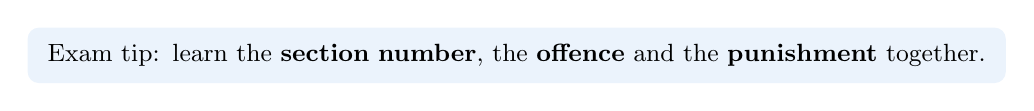
\begin{tikzpicture}
    \node[fill=sky,rounded corners,text width=12cm,align=center,font=\small,inner sep=6pt]
      {Exam tip: learn the \textbf{section number}, the \textbf{offence} and the \textbf{punishment} together.};
  \end{tikzpicture}
\end{frame}

% ------------------------------------------------------------
\begin{frame}{Indian Contract Act, 1872}
  \begin{columns}[c]
    \begin{column}{0.5\textwidth}
      \centering
      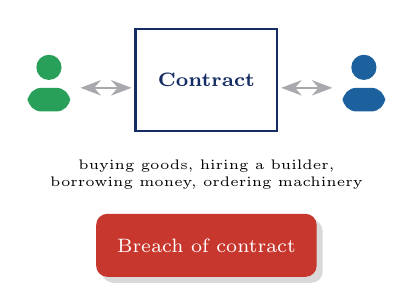
\begin{tikzpicture}
        \pic at (0,0) {person=leaf}; \pic at (4,0) {person=ocean};
        \node[draw=navy,thick,fill=white,minimum width=18mm,minimum height=13mm] (c) at (2,0.3) {};
        \node[font=\scriptsize\bfseries,text=navy] at (2,0.3) {Contract};
        \draw[<->,thick,ink!40] (0.4,0.2) -- (1.05,0.2); \draw[<->,thick,ink!40] (2.95,0.2) -- (3.6,0.2);
        \node[font=\tiny,text width=40mm,align=center] at (2,-0.9) {buying goods, hiring a builder, borrowing money, ordering machinery};
        \node[solid box=brick,minimum width=28mm,font=\scriptsize] at (2,-1.8) {Breach of contract};
      \end{tikzpicture}
    \end{column}
    \begin{column}{0.48\textwidth}
      \begin{block}{Contract}
        \small A \textbf{legally binding agreement} between two or more persons. The parties set its terms and must perform as specified.
      \end{block}
      \begin{alertblock}{Breach}
        \small Violating the terms, or not performing one's obligations.
      \end{alertblock}
      \begin{exampleblock}{Remedy 1: Damages}
        \small Compensation for loss arising \textbf{in the usual course} from the breach, not for remote or indirect loss, unless both parties knew it was likely.
      \end{exampleblock}
    \end{column}
  \end{columns}
\end{frame}

% ------------------------------------------------------------
\begin{frame}{Contract Act: More Remedies and Offshoring}
  \centering
  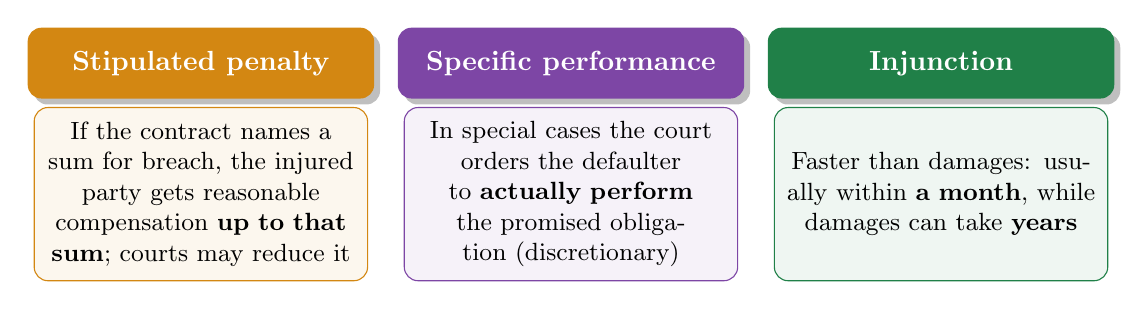
\begin{tikzpicture}
    \foreach \x/\c/\t/\d in {
      0/amber!90!black/Stipulated penalty/If the contract names a sum for breach\comma{} the injured party gets reasonable compensation \textbf{up to that sum}; courts may reduce it,
      4.7/grape/Specific performance/In special cases the court orders the defaulter to \textbf{actually perform} the promised obligation (discretionary),
      9.4/leaf!80!black/Injunction/Faster than damages: usually within \textbf{a month}\comma{} while damages can take \textbf{years}}
    {
      \node[fill=\c,text=white,rounded corners=5pt,font=\bfseries,minimum width=44mm,minimum height=9mm,drop shadow] (h) at (\x,0) {\t};
      \node[draw=\c,fill=\c!7,rounded corners=5pt,text width=40mm,minimum height=22mm,font=\small,anchor=north,align=center] at ([yshift=-1mm]h.south) {\d};
    }
  \end{tikzpicture}
  \vspace{3mm}
  \begin{block}{Offshoring to India}
    \small Foreign firms protect data and IP mainly through \textbf{contracts}. They should sign an exhaustive \textbf{Service Level Agreement (SLA)} covering data security and confidentiality.
  \end{block}
\end{frame}

% ------------------------------------------------------------
\begin{frame}{Indian Penal Code: Sections 406 and 420}
  \begin{columns}[T]
    \begin{column}{0.49\textwidth}
      \centering
      
\begin{tikzpicture}
        \node[circle,fill=grape,text=white,font=\Large\bfseries,minimum size=15mm,drop shadow] {406};
      \end{tikzpicture}\\[1mm]
      \textbf{\textcolor{grape}{Criminal breach of trust}}\\[1mm]
      {\small A person \textbf{entrusted} with property dishonestly misappropriates it, uses or disposes of it wrongfully, or induces another to do so.}\\[2mm]
      \colorbox{grape!15}{\small Up to \textbf{3 years}, or fine, or both}
    \end{column}
    \begin{column}{0.49\textwidth}
      \centering
      
\begin{tikzpicture}
        \node[circle,fill=brick,text=white,font=\Large\bfseries,minimum size=15mm,drop shadow] {420};
      \end{tikzpicture}\\[1mm]
      \textbf{\textcolor{brick}{Cheating}}\\[1mm]
      {\small Cheating and dishonestly inducing a person to \textbf{deliver property}, or to alter or destroy a valuable security.}\\[2mm]
      \colorbox{brick!15}{\small Up to \textbf{7 years} and a fine}
    \end{column}
  \end{columns}
  \vspace{4mm}
  \begin{block}{Why in a security course?}
    \small An employee who misuses entrusted data, or a fraudster who tricks people online, can be prosecuted under these sections.
  \end{block}
\end{frame}

% ------------------------------------------------------------
\begin{frame}{Indian Copyright Act: A Timeline}
  \centering
  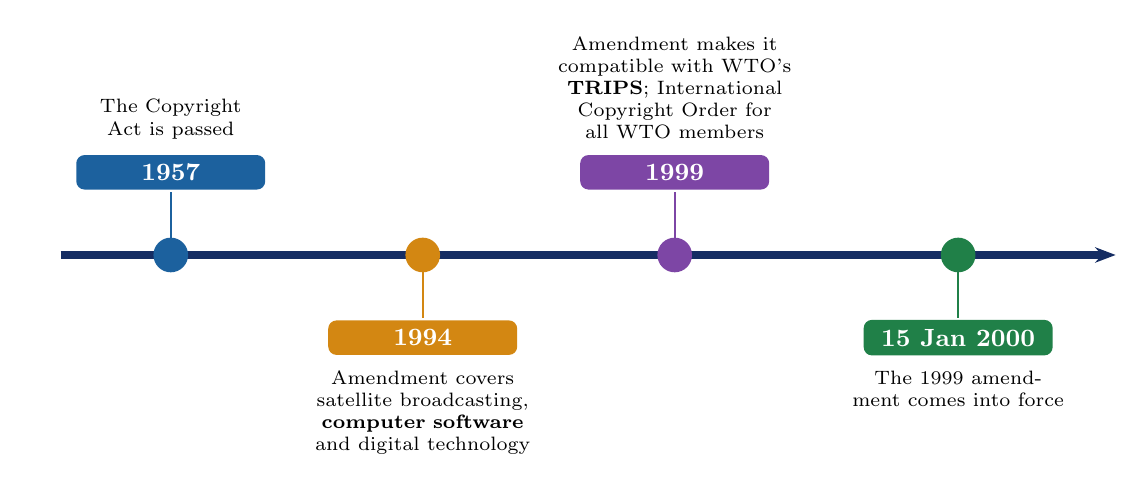
\begin{tikzpicture}
    \draw[navy,line width=3pt,->] (0,0) -- (13.4,0);
    \foreach \x/\c/\y/\t/\d in {
      1.4/ocean/1/1957/The Copyright Act is passed,
      4.6/amber!90!black/-1/1994/Amendment covers satellite broadcasting\comma{} \textbf{computer software} and digital technology,
      7.8/grape/1/1999/Amendment makes it compatible with WTO's \textbf{TRIPS}; International Copyright Order for all WTO members,
      11.4/leaf!80!black/-1/15 Jan 2000/The 1999 amendment comes into force}
    {
      \fill[\c] (\x,0) circle (2.2mm);
      \draw[\c,thick] (\x,0) -- (\x,\y*0.8);
      \node[fill=\c,text=white,rounded corners=3pt,font=\small\bfseries,minimum width=24mm] at (\x,\y*1.05) {\t};
      \ifnum\y>0 \node[font=\scriptsize,text width=34mm,align=center,anchor=south] at (\x,1.35) {\d};
      \else \node[font=\scriptsize,text width=34mm,align=center,anchor=north] at (\x,-1.35) {\d};\fi
    }
  \end{tikzpicture}
  \vspace{3mm}

  {\small India has one of the \textbf{most modern} copyright protection laws in the world. TRIPS = Trade-Related aspects of Intellectual Property Rights.}
\end{frame}

% ------------------------------------------------------------
\begin{frame}{Copyright Infringement: Section 63B}
  \begin{columns}[c]
    \begin{column}{0.48\textwidth}
      \centering
      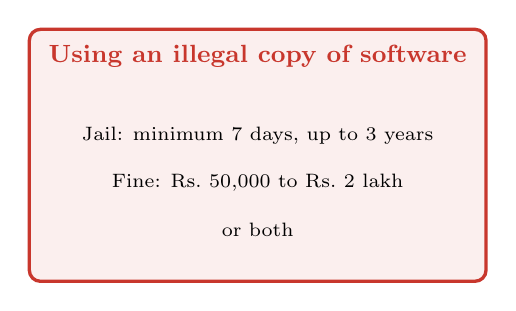
\begin{tikzpicture}
        \node[draw=brick,very thick,fill=brick!8,rounded corners,minimum width=58mm,minimum height=32mm] (b) at (0,0) {};
        \node[font=\small\bfseries,text=brick,anchor=north] at ([yshift=-1mm]b.north) {Using an illegal copy of software};
        \foreach \t/\y in {Jail: minimum 7 days\comma{} up to 3 years/0.25,Fine: Rs.\ 50\comma{}000 to Rs.\ 2 lakh/-0.35,or both/-0.95}
          \node[font=\scriptsize] at (0,\y) {\t};
      \end{tikzpicture}
    \end{column}
    \begin{column}{0.5\textwidth}
      \begin{itemize}\small\setlength{\itemsep}{4pt}
        \item Anyone who \textbf{knowingly} uses an illegal copy of a computer program can be punished under \textbf{Section 63B}
      \end{itemize}
      \begin{block}{Copyright, not patent}
        \small In India, software has \textbf{copyright} protection but \textbf{no patent} protection. A program is an algorithm, and patent law does not protect algorithms.
      \end{block}
      \begin{exampleblock}{``Software'' includes}
        \small Programs, databases, computer files, design material, and printed documentation such as user manuals.
      \end{exampleblock}
    \end{column}
  \end{columns}
\end{frame}

% ------------------------------------------------------------
\begin{frame}{Consumer Protection Act and Specific Relief Act}
  \begin{columns}[T]
    \begin{column}{0.49\textwidth}
      \centering
      
\begin{tikzpicture}
        \pic[scale=1.2] at (0,0) {person=leaf};
        \fill[leaf!20,draw=leaf,very thick] (1.6,0.9) -- (2.4,0.6) -- (2.3,-0.3) -- (1.6,-0.8) -- (0.9,-0.3) -- (0.8,0.6) -- cycle;
        \node[font=\large\bfseries,text=leaf!70!black] at (1.6,0.1) {\checkmark};
      \end{tikzpicture}\\[1mm]
      \textbf{\textcolor{leaf!70!black}{Consumer Protection Act, 1986}}\\[1mm]
      {\small In force from \textbf{15 April 1986}, to protect consumers from exploitation and poor goods and services. Consumers can complain of \textbf{``deficiency of service''}, e.g.\ disclosing their information without proper authorization.}
    \end{column}
    \begin{column}{0.49\textwidth}
      \centering
      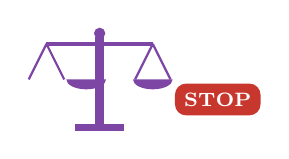
\begin{tikzpicture}
        \pic[scale=0.9] at (0,0) {scales=grape};
        \node[fill=brick,text=white,font=\scriptsize\bfseries,rounded corners] at (1.5,-0.3) {STOP};
      \end{tikzpicture}\\[1mm]
      \textbf{\textcolor{grape}{Specific Relief Act, 1963}}\\[1mm]
      {\small Under \textbf{Section 39}, a person can claim \textbf{temporary and permanent injunctions} against the unauthorized disclosure of confidential information.}
    \end{column}
  \end{columns}
\end{frame}

% ------------------------------------------------------------
\begin{frame}{Indian Laws for Information Security: Summary}
  \centering
  \renewcommand{\arraystretch}{1.45}
  \small
  \begin{tabular}{>{\bfseries}l >{\raggedright\arraybackslash}p{7.6cm}}
    \toprule
    \rowcolor{navy}\textcolor{white}{Law} & \textcolor{white}{\textbf{What it helps with}}\\
    \midrule
    \textcolor{navy}{IT Act, 2000} & Unauthorized access, virus, hacking, source-code tampering, breach of confidentiality\\
    \textcolor{ocean}{Indian Contract Act, 1872} & Breach of contract and SLAs: damages, penalty, specific performance\\
    \textcolor{grape}{Indian Penal Code} & Criminal breach of trust (406), cheating (420)\\
    \textcolor{amber!80!black}{Copyright Act, 1957} & Illegal copies of software (63B)\\
    \textcolor{leaf!70!black}{Consumer Protection Act, 1986} & Deficiency of service, such as leaking customer data\\
    \textcolor{brick}{Specific Relief Act, 1963} & Injunctions against disclosure of confidential information (Sec.\ 39)\\
    \bottomrule
  \end{tabular}
\end{frame}

% ------------------------------------------------------------
\begin{frame}{Government Initiatives: STQC}
  \begin{columns}[c]
    \begin{column}{0.48\textwidth}
      \centering
      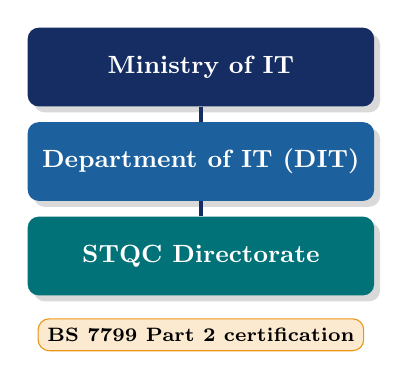
\begin{tikzpicture}
        \node[solid box=navy,minimum width=44mm,minimum height=10mm] (mit) at (0,1.4) {Ministry of IT};
        \node[solid box=ocean,minimum width=44mm,minimum height=10mm] (dit) at (0,0.2) {Department of IT (DIT)};
        \node[solid box=aqua!80!black,minimum width=44mm,minimum height=10mm,align=center] (st) at (0,-1.0) {STQC Directorate};
        \draw[navy,very thick] (mit) -- (dit) -- (st);
        \node[fill=amber!20,draw=amber,rounded corners,font=\scriptsize\bfseries] at (0,-2.0) {BS 7799 Part 2 certification};
      \end{tikzpicture}
    \end{column}
    \begin{column}{0.5\textwidth}
      \begin{block}{Standardization, Testing and Quality Certification}
        \small Set up because Indian firms needed internationally accredited security standards.
      \end{block}
      \begin{itemize}\small\setlength{\itemsep}{3pt}
        \item Launched an independent third-party certification scheme for \textbf{Information Security Management Systems} (BS 7799 Part 2)
        \item Accredited by \textbf{RvA, Netherlands}
        \item Tests hardware and software, certifies products, and \textbf{trains} people in quality and security
      \end{itemize}
    \end{column}
  \end{columns}
\end{frame}

% ------------------------------------------------------------
\begin{frame}{CERT-In: Computer Emergency Response Team}
  \centering
  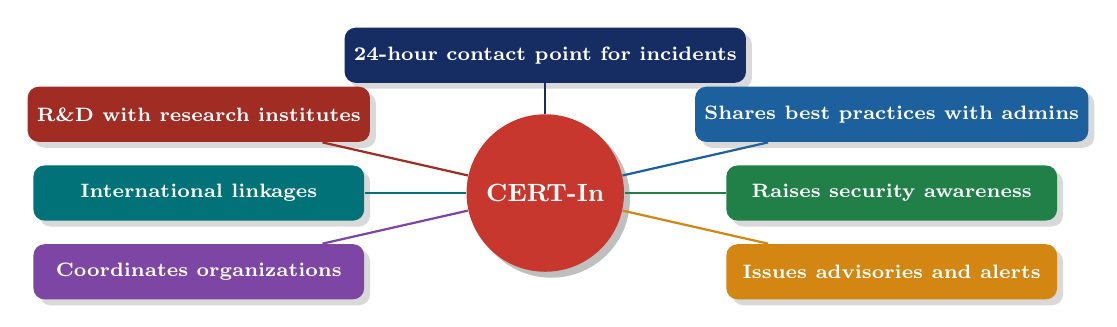
\begin{tikzpicture}
    \node[circle,fill=brick,text=white,font=\small\bfseries,minimum size=20mm,align=center,drop shadow] (c) at (0,0) {CERT-In};
    \foreach \a/\t/\c/\px/\py in {90/24-hour contact point for incidents/navy/0/1.75,38/Shares best practices with admins/ocean/4.4/1.0,-14/Raises security awareness/leaf!80!black/4.4/0,-66/Issues advisories and alerts/amber!90!black/4.4/-1.0,-114/Coordinates organizations/grape/-4.4/-1.0,-166/International linkages/aqua!80!black/-4.4/0,142/R\&D with research institutes/brick!80!black/-4.4/1.0}{
      \node[solid box=\c,minimum width=42mm,minimum height=7mm,font=\scriptsize\bfseries] (s\a) at (\px,\py) {\t};
      \draw[\c,thick] (c) -- (s\a);
    }
  \end{tikzpicture}
  \vspace{1mm}

  {\small Set up by the DIT as part of the \textbf{international CERT community}, to protect India's IT assets against viruses and other threats.}
\end{frame}

% ------------------------------------------------------------
\begin{frame}{ISTDC: Information Security Technology Development Council}
  \begin{columns}[c]
    \begin{column}{0.44\textwidth}
      \begin{block}{Objective}
        \small To \textbf{facilitate, coordinate and promote} technological advances, and respond to information security incidents, threats and attacks at the \textbf{national level}.
      \end{block}
    \end{column}
    \begin{column}{0.54\textwidth}
      \centering
      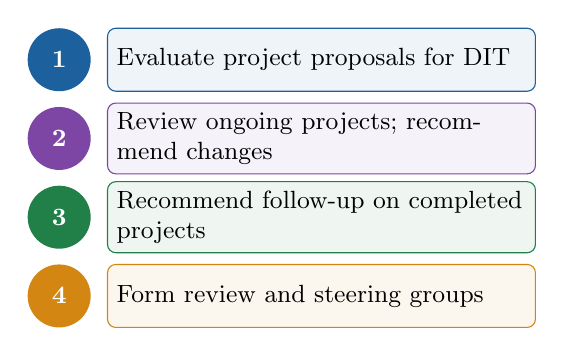
\begin{tikzpicture}
        \foreach \t/\c [count=\i from 0] in {Evaluate project proposals for DIT/ocean,Review ongoing projects; recommend changes/grape,Recommend follow-up on completed projects/leaf!80!black,Form review and steering groups/amber!90!black}{
          \node[circle,fill=\c,text=white,font=\small\bfseries,minimum size=8mm] (c\i) at (0,-\i*1.0) {\the\numexpr\i+1\relax};
          \node[draw=\c,fill=\c!7,rounded corners=3pt,anchor=west,text width=52mm,minimum height=8mm,font=\small] at ([xshift=2mm]c\i.east) {\t};
        }
      \end{tikzpicture}
    \end{column}
  \end{columns}
\end{frame}

% ------------------------------------------------------------
\begin{frame}{Legal Issues of Cryptography: Patents}
  \begin{columns}[c]
    \begin{column}{0.48\textwidth}
      \centering
      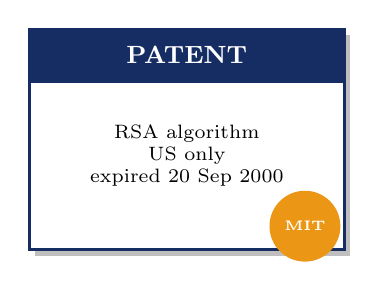
\begin{tikzpicture}
        \node[draw=navy,very thick,fill=white,minimum width=40mm,minimum height=28mm,drop shadow] (p) at (0,0) {};
        \fill[navy] ([yshift=-7mm]p.north west) rectangle (p.north east);
        \node[white,font=\small\bfseries] at ([yshift=-3.5mm]p.north) {PATENT};
        \node[font=\scriptsize,align=center] at (0,-0.2) {RSA algorithm\\US only\\expired 20 Sep 2000};
        \node[circle,fill=amber,text=white,font=\tiny\bfseries,minimum size=9mm] at (1.5,-1.1) {MIT};
      \end{tikzpicture}
    \end{column}
    \begin{column}{0.5\textwidth}
      \begin{itemize}\small\setlength{\itemsep}{3pt}
        \item The legal picture changes quickly: ``if you're going to do anything involving cryptography, \textbf{talk to a lawyer}''
        \item Most crypto techniques were \textbf{patented}, which slowed their use; being free was a key criterion for choosing \textbf{AES}
        \item \textbf{RSA}, developed at MIT, was patented only in the US, licensed by one company, until \textbf{20 September 2000}
        \item \textbf{DSS} was promoted as freely licensable, but rival patent claims (Hellman-Merkle, Schnorr) made it murky
      \end{itemize}
    \end{column}
  \end{columns}
\end{frame}

% ------------------------------------------------------------
\begin{frame}{Important Crypto Patents (All Expired)}
  \centering
  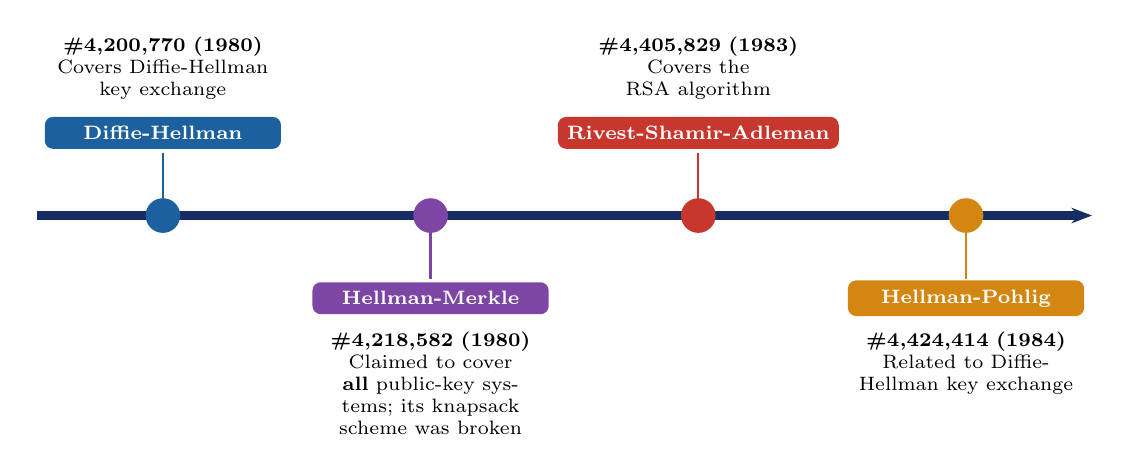
\begin{tikzpicture}
    \draw[navy,line width=3pt,->] (0,0) -- (13.4,0);
    \foreach \x/\c/\y/\t/\n/\d in {
      1.6/ocean/1/Diffie-Hellman/\#4\comma{}200\comma{}770 (1980)/Covers Diffie-Hellman key exchange,
      5.0/grape/-1/Hellman-Merkle/\#4\comma{}218\comma{}582 (1980)/Claimed to cover \textbf{all} public-key systems; its knapsack scheme was broken,
      8.4/brick/1/Rivest-Shamir-Adleman/\#4\comma{}405\comma{}829 (1983)/Covers the RSA algorithm,
      11.8/amber!90!black/-1/Hellman-Pohlig/\#4\comma{}424\comma{}414 (1984)/Related to Diffie-Hellman key exchange}
    {
      \fill[\c] (\x,0) circle (2.2mm);
      \draw[\c,thick] (\x,0) -- (\x,\y*0.8);
      \node[fill=\c,text=white,rounded corners=3pt,font=\scriptsize\bfseries,minimum width=30mm] at (\x,\y*1.05) {\t};
      \ifnum\y>0 \node[font=\scriptsize,text width=32mm,align=center,anchor=south] at (\x,1.35) {\textbf{\n}\\\d};
      \else \node[font=\scriptsize,text width=32mm,align=center,anchor=north] at (\x,-1.35) {\textbf{\n}\\\d};\fi
    }
  \end{tikzpicture}
\end{frame}

% ------------------------------------------------------------
\begin{frame}{Export Controls}
  \begin{columns}[c]
    \begin{column}{0.45\textwidth}
      \centering
      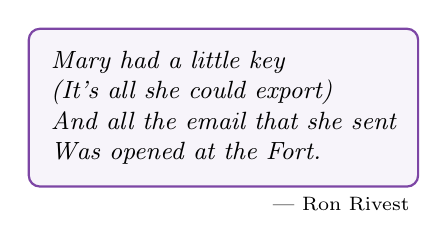
\begin{tikzpicture}
        \node[draw=grape,fill=grape!6,thick,rounded corners,font=\small\itshape,align=left,inner sep=8pt] (poem) {Mary had a little key\\(It's all she could export)\\And all the email that she sent\\Was opened at the Fort.};
        \node[font=\scriptsize,anchor=north east] at (poem.south east) {--- Ron Rivest};
      \end{tikzpicture}
    \end{column}
    \begin{column}{0.53\textwidth}
      \begin{itemize}\small\setlength{\itemsep}{4pt}
        \item The US government once placed \textbf{severe restrictions} on exporting encryption
        \item It treated encryption like a \textbf{dangerous technology}, like germ warfare or nuclear weapons
        \item Domestic products could use strong crypto, but had to \textbf{interoperate} with weak exportable ones
        \item This caused bitterness in industry, and fascinating technical designs
      \end{itemize}
      \begin{exampleblock}{Today}
        \small Export controls have now been \textbf{largely lifted}.
      \end{exampleblock}
    \end{column}
  \end{columns}
\end{frame}

% ------------------------------------------------------------
\begin{frame}{Module 5 Summary}
  \begin{columns}[T]
    \begin{column}{0.49\textwidth}
      \begin{block}{Lesson 5: Key Escrow}
        \small
        \begin{itemize}\setlength{\itemsep}{0pt}
          \item Lawful wiretaps vs.\ privacy
          \item Clipper / EES: chip ID, split key, 2 agencies
          \item Trustee protocol with $n$ trustees and a KDC
          \item Politics: few advantages, many disadvantages
        \end{itemize}
      \end{block}
    \end{column}
    \begin{column}{0.49\textwidth}
      \begin{exampleblock}{Lesson 8: Legal Issues}
        \small
        \begin{itemize}\setlength{\itemsep}{0pt}
          \item PAPA; privacy; hierarchy of regulators
          \item Digital signatures and the law
          \item IT Act 2000: Sections 43, 65, 66, 72
          \item Contract Act, IPC, Copyright, Consumer, Specific Relief
          \item STQC, CERT-In, ISTDC; patents; export controls
        \end{itemize}
      \end{exampleblock}
    \end{column}
  \end{columns}
  \vspace{1mm}
  \begin{alertblock}{Review questions}
    \scriptsize
    1.~Discuss key escrow in detail. \quad 2.~Explain the IT Act, 2000. \quad 3.~Describe the Indian Contract Act, 1872. \quad
    4.~What is the Indian Penal Code? \quad 5.~Explain the Indian Copyright Act. \quad 6.~What is the Consumer Protection Act? \quad
    7.~What initiatives has the government taken to upgrade security standards? \quad 8.~Write short notes on legal issues.
  \end{alertblock}
\end{frame}

% ------------------------------------------------------------
\begin{frame}{References}
  \begin{enumerate}\setlength{\itemsep}{8pt}
    \item William Stallings, \emph{Cryptography and Network Security}, PHI Publishers.
    \item Charlie Kaufman, Radia Perlman, \emph{Network Security}, Pearson Education.
    \item Bruce Schneier, \emph{Applied Cryptography}, John Wiley \& Sons.
    \item Roberta Bragg, \emph{Network Security: The Complete Reference}, TMH.
  \end{enumerate}
  \vspace{6mm}
  \centering
  
\begin{tikzpicture}
    \node[fill=navy,text=white,rounded corners=8pt,inner sep=10pt,font=\Large\bfseries,drop shadow] {Thank You! \; Questions?};
  \end{tikzpicture}
\end{frame}

\end{document}
